% !Mode:: "TeX:UTF-8"
% !TeX program = xelatex

\documentclass[fontset=windows,type=bachelor,campus=shenzhen,chapterbold=false,tocblank=false]{hithesisbook}

\usepackage{hithesis}

\usepackage{listings}
\usepackage{xcolor}
\usepackage{tikz}
\usepackage{tikz-timing}
\usepackage{pgfplots}
\pgfplotsset{compat=1.18}
\usepackage{amsmath}
\usepackage{amssymb}
\usepackage{booktabs}
\usepackage{array}
\usepackage{float}

% 让 listings 支持 UTF-8 输入并能在等宽段落里渲染中文注释 / 中文字符串
\usepackage{xeCJK}
\setCJKmonofont[Scale=0.92]{NSimSun}

% 代码框样式
\definecolor{codebg}{HTML}{FAFAFA}
\definecolor{codekw}{HTML}{0033B3}
\definecolor{codestr}{HTML}{067D17}
\definecolor{codecmt}{HTML}{8C8C8C}

\lstdefinestyle{codefig}{
  basicstyle=\ttfamily\small,
  keywordstyle=\color{codekw}\bfseries,
  stringstyle=\color{codestr},
  commentstyle=\color{codecmt}\itshape,
  backgroundcolor=\color{codebg},
  frame=single,
  framerule=0pt,
  rulecolor=\color{codebg},
  breaklines=true,
  breakatwhitespace=false,
  keepspaces=true,
  showstringspaces=false,
  tabsize=2,
  captionpos=b,
  extendedchars=true,
  inputencoding=utf8,
  upquote=true,
  columns=fullflexible,
  xleftmargin=8pt,
  xrightmargin=8pt,
  aboveskip=8pt,
  belowskip=8pt,
}
\lstset{style=codefig}

% 代码列表中文标号
\renewcommand{\lstlistingname}{代码}

\lstdefinelanguage{Scala}{
  morekeywords={abstract,case,catch,class,def,do,else,extends,false,final,finally,for,if,implicit,import,match,new,null,object,override,package,private,protected,return,sealed,super,this,throw,trait,true,try,type,val,var,while,with,yield,Bool,UInt,Vec,Reg,RegInit,RegEnable,Decoupled,Flipped,Output,Input,Bundle,IO,Module,Wire,when,elsewhen,otherwise},
  sensitive=true,
  morecomment=[l]{//},
  morecomment=[s]{/*}{*/},
  morestring=[b]"
}

% 图片搜索路径：本地 images/ 与 hithesis 资产目录（封面 .eps 等）
\graphicspath{{images/}{../template/latex/examples/hitbook/chinese/}}

% 行内引用空白处理（hithesis 自带）
\newcommand{\cndash}{\rule{0.2em}{0pt}\rule[0.35em]{1.6em}{0.05em}\rule{0.2em}{0pt}}

\begin{document}
\frontmatter
% !Mode:: "TeX:UTF-8"

\hitsetup{
  %===========
  % 论文类型
  %===========
  design=true,
  %
  %=====
  % 秘级
  %=====
  statesecrets={公开},
  %
  %=========
  % 中文信息
  %=========
  ctitleone={RISC-V 指令集},
  ctitletwo={乱序处理器设计},
  ctitlecover={RISC-V 指令集乱序处理器设计},
  ctitle={RISC-V 指令集乱序处理器设计},
  cxueke={工学},
  csubject={计算机科学与技术},
  caffil={深圳校区计算机科学与技术学院},
  cauthor={王靳},
  csupervisor={薛睿高级实验师},
  firstpagecdate={2026年5月},
  cdate={2026年5月15日},
  cstudentid={220111012},
  cstudenttype={本科毕业设计},
  %
  %=========
  % 英文信息
  %=========
  etitle={Design of RISC-V Out-of-Order Processor},
  exueke={Engineering},
  esubject={Computer Science and Technology},
  eaffil={\emultiline[t]{School of Computer Science and Technology \\ Shenzhen Campus}},
  eauthor={Wang Jin},
  esupervisor={Senior Experimentalist Xue Rui},
  edate={May, 2026},
  estudenttype={Bachelor of Engineering},
  %
  ckeywords={RISC-V, 乱序执行, Chisel, SoC, 差分测试},
  ekeywords={RISC-V, Out-of-Order Execution, Chisel, SoC, Difftest},
}

\begin{cabstract}

随着开源指令集架构 RISC-V 的快速发展，基于开源生态开展高性能处理器研究已成为体系结构领域的重要方向。乱序执行通过动态调度与寄存器重命名提升指令级并行性，是现代处理器获得高性能的关键机制。本文围绕“RISC-V 指令集乱序处理器设计”，完成了从核心微架构到系统软件支撑的整体实现与验证。

在微架构设计方面，本文实现了前后端解耦的单发射乱序处理器，采用统一物理寄存器的寄存器重命名方案，支持乱序执行与顺序提交，并通过重排序机制实现精确异常；前端分支预测采用 GShare+IJTC+RAS 组合方案。存储层次方面，实现了基于 VIPT 结构且采用 PLRU 替换策略的 ICache 与 DCache，以降低访存开销并兼顾地址转换场景下的访问效率。体系结构支持方面，实现了 M/S/U 三级特权架构、Sv39 虚拟内存机制与中断处理机制，为操作系统运行提供了完整硬件基础。

为保证设计正确性，本文基于 Chisel、Verilator 与 C++20 构建验证平台，结合差分测试与调试追踪工具对关键模块进行系统验证。在性能评估方面，基于 MicroBench、Dhrystone 与 CoreMark 三组基准程序并结合 RTL 寄存器与 DPI-C 事件的混合性能计数器对处理器进行了多维度定量分析：三组负载 IPC 分别为 0.47、0.45 与 0.55，\lstinline|commit / ifu_deliver| 处于 0.88--0.91 区间；Dhrystone 成绩为 0.559 DMIPS/MHz，CoreMark 成绩为 1.540 CoreMark/MHz；ICache 命中率均在 99.9996\% 以上，DCache 命中率为 96.87\%--99.99\%，分支预测命中率为 90.97\%--96.77\%。实验结果表明，所实现处理器在乱序执行、缓存访问、异常中断处理与虚拟内存管理等关键功能上均满足设计预期，并已成功运行 xv6 教学操作系统。本文工作为 RISC-V 乱序处理器的教学与工程实践提供了可复现的实现路径与系统级参考。

\end{cabstract}

\begin{eabstract}

With the rapid development of the open-source RISC-V instruction set architecture, conducting high-performance processor research within an open ecosystem has become a significant direction in computer architecture. Out-of-order execution improves instruction-level parallelism through dynamic scheduling and register renaming, serving as a key mechanism for achieving high performance in modern processors. This thesis presents a complete design and verification of a RISC-V out-of-order processor, spanning from core microarchitecture to system software support.

In terms of microarchitectural design, this work implements a single-issue out-of-order processor with a decoupled frontend-backend architecture. The processor employs a unified physical register file based register renaming scheme, supports out-of-order execution with in-order commit, and achieves precise exceptions through a reorder buffer mechanism. The frontend branch prediction adopts a combined GShare+IJTC+RAS scheme. For the memory hierarchy, VIPT-structured ICache and DCache with Pseudo-LRU replacement policy are implemented to reduce memory access latency while accommodating address translation scenarios. In terms of architectural support, M/S/U three-level privilege modes, the Sv39 virtual memory mechanism, and interrupt handling are implemented, providing a complete hardware foundation for operating system execution.

To ensure design correctness, a verification platform is built using Chisel, Verilator, and C++20, incorporating differential testing against the Spike reference model along with debugging and tracing tools for systematic module-level verification. For performance evaluation, a hybrid performance counter framework combining RTL registers with DPI-C event hooks is developed and exercised against MicroBench, Dhrystone and CoreMark benchmarks: the processor reaches IPC values of 0.47, 0.45, and 0.55 across the three workloads, with \lstinline|commit / ifu_deliver| in the 0.88--0.91 range; it achieves 0.559 DMIPS/MHz on Dhrystone and 1.540 CoreMark/MHz on CoreMark, with ICache hit rates above 99.9996\%, DCache hit rates of 96.87\%--99.99\%, and branch-prediction hit rates of 90.97\%--96.77\%. Experimental results demonstrate that the implemented processor meets design expectations across all key functionalities including out-of-order execution, cache access, exception and interrupt handling, and virtual memory management. The processor has successfully booted the xv6 teaching operating system. This work provides a reproducible implementation path and system-level reference for RISC-V out-of-order processor education and engineering practice.

\end{eabstract}

\makecover
\tableofcontents

\mainmatter
% !Mode:: "TeX:UTF-8"

\chapter[绪论]{绪~~论}

\section{研究背景、目的和意义}

\subsection{研究背景}

RISC-V 作为开源、模块化、可扩展的指令集架构~\cite{patterson2017riscv}，正在从学术研究走向产业化部署。华为发布了基于 RISC-V 的 Hi3861 开发系统~\cite{huawei2021hi3861}，NVIDIA 于 2024 年出货超十亿颗 RISC-V 核心~\cite{nvidia2024riscv}，国内政策层面亦明确鼓励 RISC-V 生态建设~\cite{china2025riscv}。相较于传统封闭指令集，RISC-V 在授权成本、生态开放性和可定制能力方面具有显著优势，为高校和科研机构开展处理器全栈设计提供了可行路径。与此同时，面向高性能场景的处理器普遍依赖乱序执行技术来提升指令级并行性和流水线吞吐率，因此围绕 RISC-V 乱序处理器开展研究具有明确的工程价值与教学价值。

从教学与科研实践看，当前公开资料中存在“简单顺序核容易入门、工业级乱序核复杂度过高”的鸿沟，不利于学习者系统理解乱序执行关键机制。蜂鸟 E203~\cite{hbirdv2} 等开源核聚焦于顺序执行，而 SonicBOOM~\cite{zhao2020sonicboom} 与香山~\cite{wang2023xiangshan} 等高性能乱序核的复杂度远超教学场景。国内已有多部教材对顺序流水线处理器设计进行了系统介绍~\cite{lei2014cpu}~\cite{wang2021cpudesign}，姚永斌的《超标量处理器设计》\cite{yao2014superscalar} 则对乱序微架构理论进行了深入讲解。然而在“理论教材”与“工业级开源核”之间，缺少一款规模适中、结构清晰、可在课堂与个人项目中完整复现的乱序处理器实现。

\subsection{研究目的}

针对上述教学与工程实践之间的断层，本文的研究目的是：以可实现、可验证、可复现为导向，设计并实现一款面向教学与工程过渡场景的 RISC-V 单发射乱序处理器及配套 SoC 平台，并通过统一的仿真验证框架对其功能正确性与性能表现进行系统评估。具体而言，本文希望达成以下目标：第一，在微架构层面打通“前端取指—分支预测—乱序发射—延迟执行—顺序提交”的完整数据通路，使学习者能够从单一代码库中观察到乱序流水线各关键机制的工作过程；第二，在系统层面提供处理器核以外的总线、存储控制器与外设支撑，使所设计的处理器具备运行真实操作系统的能力；第三，在验证层面构建以差分测试为核心、配合追踪与快照回放的仿真平台，确保所有结论可由实验数据支撑，而非仅停留于设计描述。

\subsection{研究意义}

从产业需求看，掌握高性能处理器核心微架构的自主设计能力，是推进自主可控芯片技术体系建设的重要基础~\cite{csia2024report}。本文围绕 RISC-V 乱序处理器开展的全栈设计与验证工作，对填补“教学顺序核”与“工业乱序核”之间的实现空白具有直接的教学价值；同时，本文所建立的“微架构 + SoC + 仿真验证”一体化实现路径，可为高校体系结构课程、个人项目以及后续的乱序核研究提供可复用的工程参考与实验基础。

\section{国内外研究现状}

\subsection{乱序执行理论框架的形成与完善}

20 世纪 90 年代是现代乱序处理器理论体系系统化的关键时期。Smith 与 Sohi 在 1995 年的综述~\cite{smith1995superscalar} 中指出，高性能超标量处理器的核心任务是在保持顺序语义可见性的前提下，将程序中的潜在并行性转化为硬件可执行的并行操作。该综述将处理流程归纳为取指与分支处理、寄存器相关性分析、动态发射与执行、访存数据通信、按程序顺序提交与精确中断支持等关键阶段，为后续乱序微架构设计提供了统一分析框架。

\subsection{精确异常的实现路径}

为在乱序执行条件下保持体系结构可见状态的顺序一致性，精确异常机制是核心设计点。典型实现路径包括：基于重排序缓冲区（ROB, Reorder Buffer）的顺序提交方案~\cite{smith1988precise}（在提交点统一更新架构状态）；基于 walk-back 的恢复方案（异常时按记录回退未提交状态）；基于 checkpoint 的快速恢复方案~\cite{hwu1987checkpoint}（保存关键映射快照并在错误路径上快速回滚）。三类方案分别在硬件开销、恢复时延与实现复杂度之间进行权衡。

\subsection{寄存器重命名机制与 WAW/WAR 消解}

为消除 WAW/WAR 等伪相关并释放指令级并行性，重命名机制形成了多条技术路线。第一类是 ROB-based 方案，结果先写入 ROB 项并在提交时回写架构寄存器；第二类是 Arch Register File + Future File 方案，将提交态与推测态分离管理；第三类是统一物理寄存器文件（PRF, Physical Register File）方案，通过寄存器别名表（RAT, Register Alias Table）维护映射关系并在提交后回收旧物理寄存器。统一 PRF 方案因扩展性与实现弹性较好，在 Alpha 21264~\cite{kessler1999alpha}、MIPS R10000~\cite{yeager1996r10000} 等经典乱序处理器中应用广泛。

\subsection{分支预测与前端指令供应能力提升}

分支预测能力直接决定前端取指带宽的有效利用率。相关技术从静态预测与一/二位饱和计数器，发展到两级自适应预测（如 GShare、GSelect）\cite{mcfarling1993combining}，再到混合预测与锦标赛选择机制~\cite{razilov2024tage}。同时，分支目标缓冲器（BTB, Branch Target Buffer）、返回地址栈（RAS, Return Address Stack）与间接跳转目标缓存（IJTC, Indirect Jump Target Cache）等结构被联合用于覆盖条件分支、函数返回与间接跳转场景。随着乱序窗口扩大与流水线加深，分支预测准确率与误判恢复代价已成为影响处理器实际吞吐率的关键因素。

\subsection{开源 RISC-V 与 Chisel 驱动下的新发展}

近年来，RISC-V 开源生态显著降低了高性能处理器研究的实现门槛，推动了乱序处理器从“理论可讲”向“工程可复现”转变。以 BOOM~\cite{zhao2020sonicboom}、香山~\cite{wang2023xiangshan} 等项目为代表的开源实践展示了乱序处理器在现代开源工具链下的系统化实现路径，也为后续研究提供了可参考的架构与验证经验。

同时，Chisel~\cite{bachrach2012chisel} 等硬件构造语言的发展，使复杂微架构与系统级芯片（SoC, System on Chip）集成的参数化设计、模块复用和工程维护能力明显提升。与之配套的差分测试方法~\cite{you2025difftest}（如基于 Spike~\cite{spike2026} 的逐指令对比）进一步提高了功能验证效率，形成了“设计—验证—迭代”闭环。上述新发展使得在课程与科研场景中实现具备完整特权架构、缓存与虚拟内存支持的乱序处理器成为现实可行的工程目标。

\section{本文的主要研究内容}

围绕上述理论与工程发展脉络，本文以“RISC-V 指令集乱序处理器设计”为核心，针对教学与工程过渡场景下的乱序处理器实现需求，开展以下研究内容：

\begin{enumerate}
  \item 研究面向乱序处理器的 SoC 系统级集成方案，建立处理器核、总线互连、多层次存储与外设协同工作的系统级平台架构。
  \item 研究基于 Chisel~\cite{bachrach2012chisel} 的关键知识产权核（IP, Intellectual Property Core）参数化实现方法，针对 SDRAM 控制器、Flash 控制器（串行外设接口（SPI, Serial Peripheral Interface）模式，配合就地执行（XIP, eXecute In Place）控制器实现直接取指执行）与 PSRAM 控制器（支持四线串行外设接口（QSPI, Quad SPI）与四线并行 I/O（QPI, Quad Peripheral Interface）模式及相互切换）展开存储控制器设计研究。
  \item 研究单发射乱序处理器微架构设计方法，重点围绕统一物理寄存器重命名方案、乱序执行与顺序提交流水线、以及精确异常支持机制展开。
  \item 研究基于虚拟索引物理标记（VIPT, Virtually Indexed Physically Tagged）\cite{cekleov1997vipt} 结构且采用伪最近最少使用（PLRU, Pseudo Least Recently Used）替换策略的指令缓存（ICache, Instruction Cache）与数据缓存（DCache, Data Cache）设计方法。
  \item 研究 RISC-V M/S/U 三级特权架构与 Sv39 虚拟内存机制~\cite{riscv2024priv} 在所设计处理器上的实现路径，使其具备运行操作系统所需的体系结构支持能力。
  \item 研究 NVBoard（NJU Virtual Board）\cite{nvboard2024} 在仿真平台中的集成方法，实现外设的可视化交互。
  \item 研究 xv6~\cite{cox2024xv6} 教学操作系统在所设计处理器上的移植与运行验证方法。
  \item 研究基于混合性能计数器（RTL 寄存器 + DPI-C 事件）的多维度性能评估方法，依托 MicroBench~\cite{microbench2024}、Dhrystone~\cite{weicker1984dhrystone} 与 CoreMark~\cite{coremark2009} 三组负载，对所设计处理器进行 IPC、缓存命中率、分支预测命中率等指标的定量分析。
\end{enumerate}

% !Mode:: "TeX:UTF-8"

\chapter{SoC 系统设计思路}

\section{设计目标与总体原则}

本课题 SoC 设计的核心目标是为乱序处理器提供可运行操作系统的完整系统环境，并在保证可调试性的前提下兼顾性能与实现复杂度。为此，系统采用“分层总线 + 多层次存储 + 可视化外设联调”的总体思路：高速访存路径优先保障带宽与时延，低速外设路径优先保障协议兼容与工程可维护性，同时通过统一验证框架降低系统集成阶段的调试成本。

在实现策略上，SoC 结构遵循模块化和可替换原则。处理器核、总线互连、存储控制器和外设控制器通过标准接口连接，使得各模块可以独立迭代。该设计既满足当前单发射乱序处理器的系统集成需求，也为后续微架构升级和外设扩展预留了接口空间。

\section{分层总线架构设计}

SoC 采用高级可扩展接口 4（AXI4, Advanced eXtensible Interface 4）\cite{math2012axi4} 与高级外设总线（APB, Advanced Peripheral Bus）组合的分层互连架构，以匹配不同设备的速率特征。处理器核心通过 AXI4 主接口接入一级 Crossbar，一级 Crossbar 重点服务主存访问关键路径，仅挂接高带宽存储控制器；二级 Crossbar 连接片上存储与桥接模块，承担中速设备访问；低速外设统一通过 AXI4ToAPB 桥进入 APB 域，由 APB Fanout 完成地址分发。

SoC 整体互连架构如图~\ref{fig:soc-arch} 所示。

\begin{figure}[H]
  \centering
  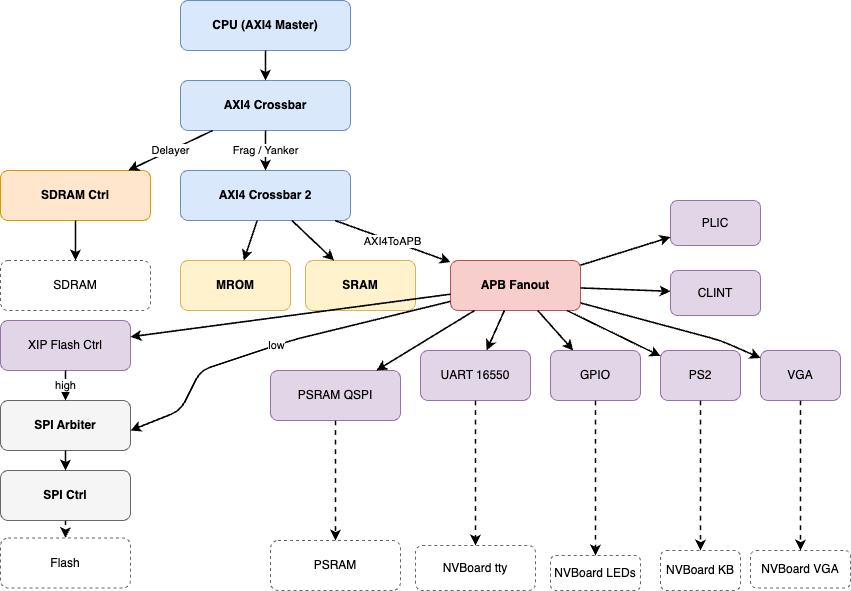
\includegraphics[width=0.95\textwidth]{soc-arch.png}
  \caption{SoC 系统整体互连架构}
  \label{fig:soc-arch}
\end{figure}

如图~\ref{fig:soc-arch} 所示，SoC 整体互连分为三个速率域。处理器核心作为唯一的 AXI4 Master 接入一级 AXI4 Crossbar。一级 Crossbar 的左侧分支经 AXI4 Delayer（用于在仿真中注入可配置的访存延迟）连接 SDRAM Controller，右侧分支经 AXI4 Fragmenter（将突发传输拆分为单拍事务以适配不支持 Burst 的从设备）与 AXI4 UserYanker（剥离用户自定义信号以对齐接口宽度）连接二级 AXI4 Crossbar。SDRAM 直接挂载在一级 Crossbar 上，以最短路径获得最高带宽。

二级 Crossbar 下挂 MROM（存放 FSBL, first stage boot loader）、SRAM（低延迟片上存储）以及 AXI4ToAPB 总线桥。总线桥将 AXI4 事务转换为 APB 协议后，由 APB Fanout 按地址空间分发至各低速外设：XIP Flash Controller、PSRAM QSPI Master、UART 16550、GPIO、PS2 键盘控制器、VGA 显示控制器，以及 PLIC（外部中断控制器）和 CLINT（定时器与软件中断控制器）。

在 Flash 访问路径上，XIP Flash Controller 与 APB Fanout 共享底层 SPI Controller 的物理访问权，通过 SPI Arbiter 进行仲裁：XIP 以高优先级发起 SPI 事务用于直接取指执行，APB 以低优先级提供 SPI 寄存器的直接读写通道。各外设控制器的 TX/RX 或数据端口连接至 NVBoard 虚拟开发板对应的外设仿真（串口终端、LED/数码管、键盘、VGA 显示器），以虚线表示。

该分层设计的关键收益在于：其一，高速域与低速域解耦，SDRAM 路径不受慢设备干扰；其二，AXI4 突发与并发事务能力被主存路径充分利用，APB 侧保持实现简单、硬件开销低；其三，桥接与仲裁逻辑集中管理，扩展新外设只需在 APB Fanout 中追加地址映射。

\section{多层次存储与启动链路设计}

存储系统采用 MROM、SRAM、Flash、PSRAM、SDRAM 的多层次组织。MROM 用于放置最小启动代码，SRAM 提供低延迟片上存储，Flash 提供非易失程序镜像并支持 XIP，PSRAM 与 SDRAM 提供更大容量主存。不同存储介质按“启动可靠性—访问延迟—容量”进行功能分工，形成从上电到系统运行的连续存储支撑。

在控制器实现上，关键 IP 核采用 Chisel~\cite{bachrach2012chisel} 实现或重写：SDRAM 控制器面向 AXI4 高带宽路径进行流水化组织，Flash/PSRAM 相关控制器面向 SPI/QSPI/QPI 协议兼容设计。Flash 访问同时支持寄存器方式与 XIP 方式，并通过仲裁机制共享底层 SPI 资源。该设计兼顾了启动阶段可执行性与运行阶段访存效率。

启动链路采用分级引导思路：上电后从 Flash 中的引导入口执行，完成基础初始化后将后续引导或系统镜像加载至 SDRAM，再跳转进入运行态。该流程减少了直接从串行 Flash 执行大体量程序的性能损失，为操作系统（如 xv6~\cite{cox2024xv6}、RT-Thread~\cite{yi2023rtthread}）启动提供更稳定的执行环境。

\begin{figure}[H]
  \centering
  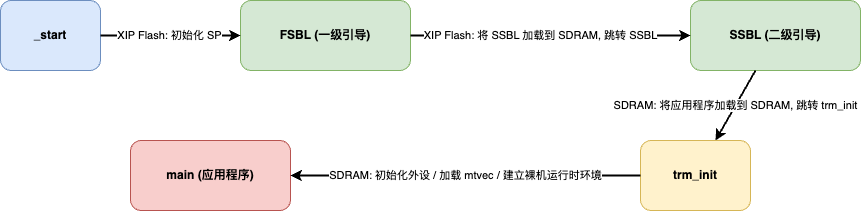
\includegraphics{boot-flow.png}
  \caption{启动链路流程图}
  \label{fig:boot-flow}
\end{figure}

\section{外设集成与可视化验证思路}

外设侧围绕“可用、可测、可观测”进行设计。UART、GPIO、PS2、VGA 等控制器通过 APB 域接入，保证接口一致性与调试便利性。针对教学与开发场景，系统进一步集成 NVBoard，将串口回显、按键输入、数码管显示与 VGA 输出纳入同一仿真闭环，使 SoC 级功能验证从单纯日志比对扩展为可交互的行为验证。

在验证方法上，SoC 联调与指令级差分测试协同使用：差分测试用于保证体系结构状态正确性，NVBoard 与外设交互用于暴露系统级时序和接口问题，二者互补提升了复杂问题定位效率。基于该思路，系统能够稳定支撑操作系统运行与外设协同工作。

\section{本章小结}

本章从目标约束、总线分层、存储组织、启动链路与外设验证五个方面阐述了 SoC 设计思路。通过 AXI4/APB 分层互连、多层次存储分工、关键控制器 Chisel 化实现以及 NVBoard 可视化联调，系统在性能、可维护性与可验证性之间取得了平衡，为乱序处理器运行 xv6 等操作系统提供了完整平台基础。

% !Mode:: "TeX:UTF-8"

\chapter{关键 IP 核设计与实现}

SoC 系统中的存储控制器直接影响系统启动流程与运行期访存性能。本章围绕 Flash 控制器、PSRAM QSPI Master 控制器与 SDRAM 控制器三个关键 IP 核，分别阐述设计方案与验证方法。

\section{Flash 控制器与 XIP 机制}

Flash 存储器通过 SPI 协议接入系统。SPI Master 选用 OpenCores 开源 IP 核~\cite{opencores_simple_spi}，基于 Wishbone 总线接口~\cite{wishbone_b4}，本课题使用 Chisel 实现了 APB-to-Wishbone 的薄封装层以接入 SoC 的 APB 域。

系统为 Flash 提供两种访问方式。第一种是命令方式：通过 APB Fanout 经 SPI Arbiter 直接读写 SPI 控制器寄存器，适用于 Bootloader 阶段的 Flash 编程与配置操作，如代码~\ref{lst:flash-read-sw} 所示。第二种是 XIP（eXecute In Place）方式：XIP 控制器将处理器对 Flash 地址窗口的 MMIO 读请求自动转换为底层 SPI 命令字序列（如读命令、地址发送与数据回传），从而以硬件方式完成“取指驱动”，其状态机流程如图~\ref{fig:xip-fsm} 所示。引入该机制的动机是避免启动阶段的“鸡生蛋”死锁：若程序存放在 Flash 中而访问 Flash 又依赖软件驱动，则驱动本身也需要先从 Flash 取出，系统将无法启动。通过 XIP 的硬件读通路，处理器无需先运行 SPI 软件驱动即可直接从 Flash 取指执行。两种方式通过 SPI Arbiter 共享物理 SPI 控制器，XIP 具有更高的仲裁优先级。

\begin{lstlisting}[language=C,caption={SPI Flash 软件轮询读取实现示例},label={lst:flash-read-sw}]
void spi_wait_done(void) {
  while (REG32(SPI_CTRL) & SPI_CTRL_GO)
    ;
}
void flash_select(void) { REG32(SPI_SS) = FLASH_SS; }
void flash_deselect(void) { REG32(SPI_SS) = 0; }

// [ 0, cmd, addr, data ]
// high                low
// Tx3                 Tx0
// Rxx 与 Txx 其实是同一个寄存器
uint32_t flash_read_word(uint32_t addr) {
  flash_select();
  REG32(SPI_TX1) = (FLASH_CMD_READ << 24) | (addr & 0x00FFFFFF);
  REG32(SPI_TX0) = 0;
  REG32(SPI_CTRL) = SPI_CTRL_CHAR_LEN(64) | SPI_CTRL_ASS
                  | SPI_CTRL_GO;
  spi_wait_done();
  uint32_t data = REG32(SPI_RX0);
  flash_deselect();
  return data;
}
\end{lstlisting}

\begin{figure}[H]
  \centering
  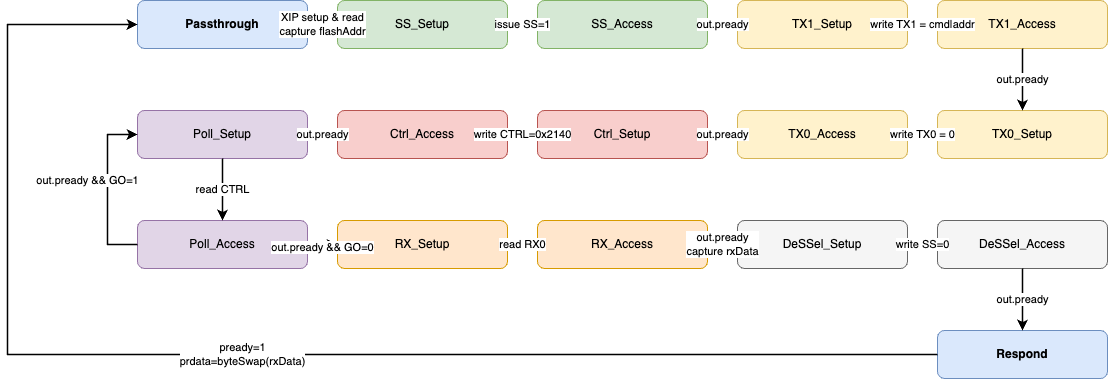
\includegraphics{xip-fsm.png}
  \caption{APB XIP 控制器状态转移图}
  \label{fig:xip-fsm}
\end{figure}

如图~\ref{fig:xip-fsm} 所示，XIP 读事务从 \lstinline|Passthrough| 状态进入后，依次经历 \lstinline|SS| 选通、\lstinline|TX1/TX0| 发送命令与地址、\lstinline|CTRL| 启动传输、\lstinline|Poll| 轮询完成、\lstinline|RX| 回读数据、\lstinline|DeSSel| 取消片选，最终在 \lstinline|Respond| 状态向上游 APB 返回读结果。

在仿真验证方面，参照 Winbond W25Q128JVSIQ 手册中的时序与命令字规范，实现了 Flash 芯片的行为级仿真模型，并通过类 UVM 的验证测试确保协议兼容性。该仿真模型的协议正确性意味着上板或流片时可直接对接物理 Flash 芯片。

\section{PSRAM QSPI Master 控制器}

PSRAM 通过 QSPI/QPI 协议接入系统，用于提供主存扩展。本课题参考 OpenCores SPI 设计思路，使用 Chisel 重新实现了完整的 QSPI Master 控制器，采用 APB 接口，支持从标准 QSPI 模式切换到 QPI 模式（四线半双工）。

\begin{figure}[H]
  \centering
  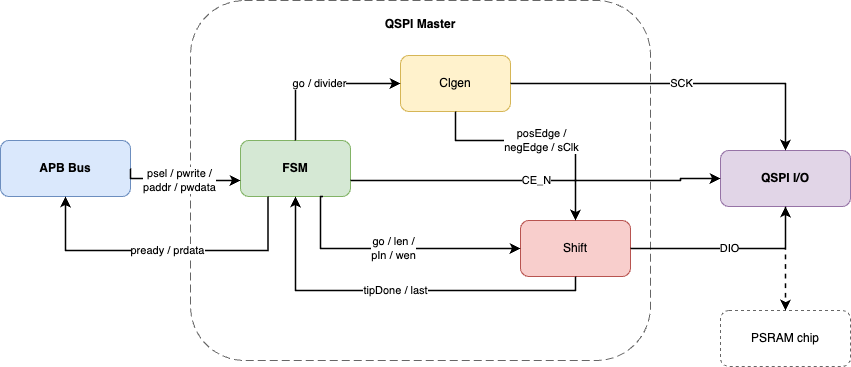
\includegraphics{qspi-arch.png}
  \caption{QSPI Master 控制器内部架构}
  \label{fig:qspi-arch}
\end{figure}

如图~\ref{fig:qspi-arch} 所示，控制器内部由三个子模块构成：状态机（FSM）负责协调 APB 总线事务与 SPI 传输流程；时钟分频器（Clgen）根据配置的分频系数生成 SPI 时钟，并向移位寄存器提供采样与驱动边沿信号；移位寄存器（Shift）在 Clgen 提供的时钟边沿驱动下完成数据的串并转换。FSM 通过 go 信号启动一次传输，Shift 在传输完成后通过 tipDone/last 信号通知 FSM，FSM 随即向 APB 侧返回 pready 完成握手。

在仿真验证方面，参照 ISSI IS66WVS4M8ALL/BLL 手册~\cite{issi_is66wvs4m8} 中的命令字与时序规范，实现了 PSRAM 颗粒的行为级仿真模型\footnote{项目仓库：\url{https://github.com/KINGFIOX/spi-master}}，用于在 Verilator 仿真环境中验证 QSPI 控制器的协议正确性。

\section{SDRAM 控制器}

为提供较大容量的主存储空间，SDRAM 控制器挂载在一级 AXI4 Crossbar 上。本课题参考 ultraembedded 开源的 SDRAM 控制器~\cite{ultraembedded_sdram}（Verilog 实现），使用 Chisel 进行了完整重写\footnote{项目仓库：\url{https://github.com/KINGFIOX/core_sdram_axi4}}，以实现参数化扩展并与 SoC 其他 Chisel 模块统一维护。重写后的控制器利用 Chisel 内置的 Queue 模块对请求和响应通路进行解耦，流水化程度高于原始 Verilog 版本。

控制器支持位扩展与字扩展两种组织方式。位扩展模式下，将两颗 SDRAM 芯片与同一个 SDRAM Core 组成一个 Bank，对同一行/列命令进行同步激活与访问，将两颗粒各自输出的 16bit 数据在控制器侧拼接为 32bit 数据通路。字扩展模式下，两个 SDRAM Core 以低位交叉（Low-order Interleaving）方式并联，按地址低位将请求映射到奇偶 Core：一个 Core 处理偶字，另一个 Core 处理奇字。

\begin{figure}[H]
  \centering
  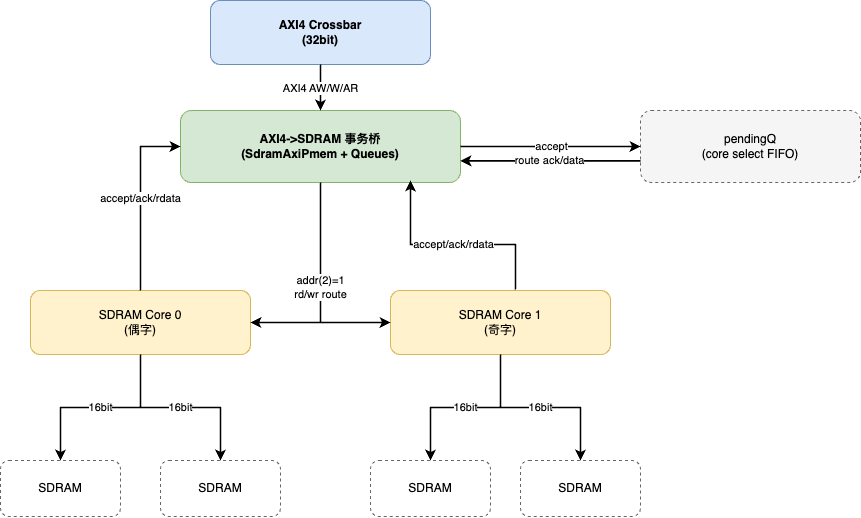
\includegraphics{sdram-interleave.png}
  \caption{SDRAM 控制器字扩展与低位交叉架构}
  \label{fig:sdram-interleave}
\end{figure}

如图~\ref{fig:sdram-interleave} 所示，图中的中间模块本质上是 AXI4 到 SDRAM Core 接口的事务桥。该桥将 AXI4 总线事务转换为 Core 请求信号，并依据地址位（\lstinline|addr(2)|）在两个 Core 间进行路由；请求被目标 Core 接收后，将 Core 选择信息写入 pending FIFO，后续再按 FIFO 记录回收对应 Core 的 \lstinline|ack/readData/error| 响应并返回 AXI4 侧。该机制既支持低位交叉并发访问，也保证了响应回传与请求顺序的一致性。

在仿真验证方面，参照 Micron MT48LC16M16A2 手册~\cite{micron_mt48lc16m16a2} 实现了 SDRAM 颗粒的行为级仿真模型，准确模拟了 ACTIVATE、READ、WRITE、PRECHARGE、AUTO REFRESH 等命令的时序行为。验证平台采用基于 SystemC~\cite{ieee2011systemc} 的 UVM 架构，整体框图如图~\ref{fig:sdram-tb} 所示。

\begin{figure}[H]
  \centering
  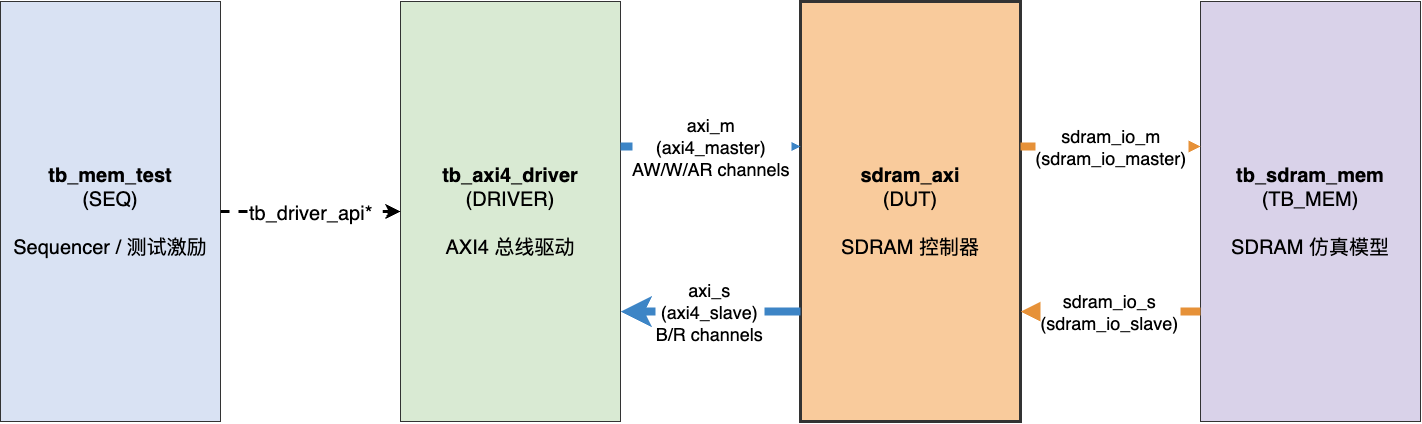
\includegraphics{sdram-testbench.png}
  \caption{SDRAM AXI4 Testbench 硬件框图}
  \label{fig:sdram-tb}
\end{figure}

该测试平台由四个模块组成。tb\_mem\_test（SEQ）作为 Sequencer 负责产生测试激励，包括随机地址、数据长度与突发模式等参数，并通过 tb\_driver\_api 接口传递给 tb\_axi4\_driver（DRIVER）。tb\_axi4\_driver 将测试激励转换为符合 AXI4 协议的总线事务，通过 axi\_m（axi4\_master）接口向 DUT 发起 AW/W/AR 通道请求，并从 axi\_s（axi4\_slave）接口接收 B/R 通道响应。sdram\_axi（DUT）即待测的 SDRAM 控制器，接收 AXI4 事务并将其转换为 SDRAM 物理接口时序，通过 sdram\_io\_m（sdram\_io\_master）接口驱动下游存储模型。tb\_sdram\_mem（TB\_MEM）为 SDRAM 芯片的行为级仿真模型，通过 sdram\_io\_s（sdram\_io\_slave）接口响应控制器发出的命令序列。

\section{本章小结}

本章介绍了 SoC 中三个关键存储控制器的设计与验证。Flash 控制器通过 SPI Arbiter 同时支持命令访问与 XIP 直接取指执行；PSRAM QSPI Master 以 FSM + Clgen + Shift 三模块架构实现 QSPI/QPI 协议兼容；SDRAM 控制器通过 Chisel 重写实现了流水化与低位交叉字扩展。三个控制器均配有行为级仿真模型并通过协议级验证，具备直接对接物理芯片的能力。

% !Mode:: "TeX:UTF-8"

\chapter{前后端解耦架构}

\section{前后端解耦架构设计}

本文实现的乱序处理器采用前后端解耦架构。前端（FrontEnd）负责取指与分支预测，后端（BackEnd）负责译码、寄存器重命名、分派、发射、执行、写回、晚执行、提交。前后端之间通过一个指令队列（Instruction Queue）进行缓冲与解耦，后端在需要冲刷流水线时通过 flush 信号同步清空该队列，分支预测失败或异常恢复时通过 redirect 信号将正确的 PC 反馈给前端。

\begin{figure}[H]
  \centering
  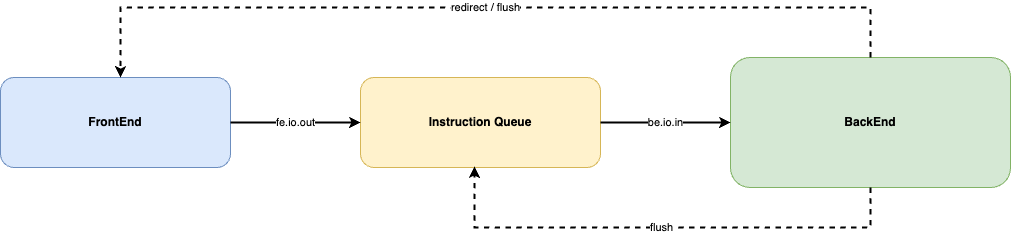
\includegraphics{fe-be-arch.png}
  \caption{前后端解耦架构与指令队列}
  \label{fig:fe-be-arch}
\end{figure}

如图~\ref{fig:fe-be-arch} 所示，前端产生的指令流经指令队列缓冲后进入后端；后端在检测到分支预测错误或异常时，通过 flush 信号清空队列中的无效指令，同时通过 redirect 信号将恢复后的目标 PC 发送给前端，使前端从正确地址重新开始取指。

\section{前后端解耦架构的含义}

前后端解耦的含义体现在时序解耦与实现解耦两个层面，并由此带来弹性的设计空间。

在时序解耦方面，前后端之间的连接方式是可配置的：既可以选择点对点直连（组合逻辑穿透，零周期延迟），也可以插入深度可调的缓冲队列。当使用队列时，前后端各自按自身节奏运行——后端因数据依赖或功能单元冲突暂停消费时，前端仍可继续取指填充队列，避免取指带宽浪费；前端遭遇 ICache 缺失时，后端可继续执行队列中已缓冲的指令，减少流水线气泡。队列深度作为参数，可根据实际时序需求灵活调整。

在实现解耦方面，前端与后端通过标准 ready-valid 握手协议通信，两侧的内部实现完全独立。前端既可以采用流水化结构，也可以完全使用软件实现。在开发过程中，硬件前端由于需要等待总线响应与 ICache 缺失处理，指令供应速率有限，后端负载偏低，难以充分暴露乱序流水线在高压力下的时序问题。为此，本课题利用解耦架构的可替换性，在前端内嵌入 Spike 参考模型：Spike 每执行一条指令即可获得精确的下一条指令 PC，使分支预测几乎 100\% 正确，同时取指不经过总线，几乎每个周期都能向后端供应一条有效指令。这一做法相当于对后端进行了满载压力测试，成功暴露了一个在常规硬件前端下因指令供应不足、未形成反压（back-pressure）而被隐藏的 bug——该 bug 表现为反压条件下数据转发时机错过，仅在后端持续满载时才会触发。定位并修复该问题后，前端切换回正常硬件实现。图~\ref{fig:spike-frontend} 展示了使用 Spike 软件前端运行 MicroBench 测试套件的结果：全部测试项通过，共提交 624375 条指令，其中 142230 条分支指令仅产生 514 次预测错误，命中率达 99.64\%，验证了该方案的指令供应充分性。这一经验表明，解耦架构不仅降低了模块间的开发耦合度，还为针对性的压力测试提供了灵活的验证手段。

\begin{figure}[H]
  \centering
  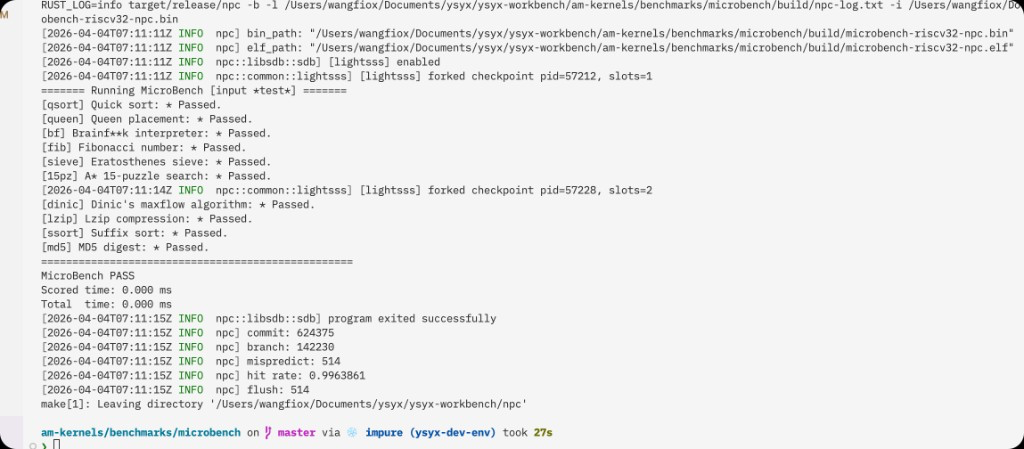
\includegraphics{spike-frontend-bench.png}
  \caption{Spike 软件前端运行 MicroBench 的测试结果（分支预测命中率 99.64\%）}
  \label{fig:spike-frontend}
\end{figure}

\section{本章小结}

弹性设计空间是解耦架构的另一直接收益。指令队列作为缓冲层，使得前端分支预测器或取指流水线的升级不影响后端接口，有利于微架构的增量迭代与独立优化。

% !Mode:: "TeX:UTF-8"

\chapter{前端：取指单元与动态分支预测设计}

前端负责为后端持续供应有效指令，其内部由取指单元（IFU, Instruction Fetch Unit）与分支预测单元（Predict）两个子模块组成。IFU 采用 4 段流水结构完成地址翻译与 ICache 访问，Predict 对当前取到的指令进行轻量译码并输出预测的下一条指令 PC，两者协同工作形成“取指—预测—下一轮取指”的闭环。

\begin{figure}[H]
  \centering
  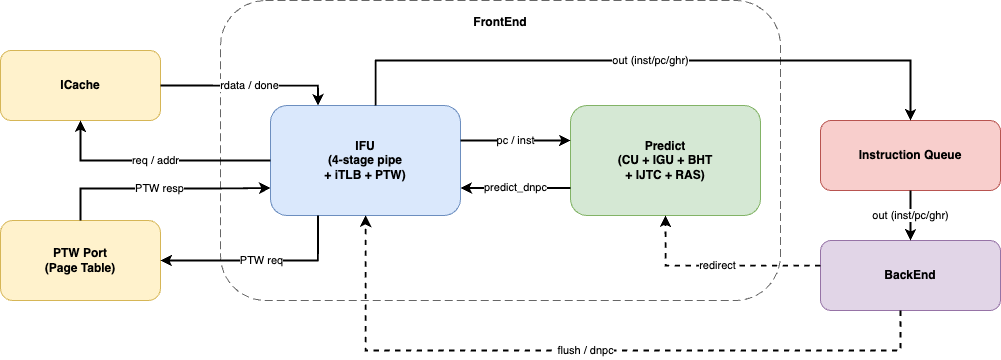
\includegraphics{frontend-arch.png}
  \caption{前端内部架构与外部接口}
  \label{fig:frontend-arch}
\end{figure}

如图~\ref{fig:frontend-arch} 所示，IFU 通过 ICache 端口和 PTW(page table walker) 端口分别访问指令缓存与页表，取到的指令与 PC 传递给 Predict 进行分支预测，Predict 返回预测的下一条 PC 供 IFU 在下一轮取指时使用。IFU 的输出（指令、PC、预测信息）经指令队列送入后端。后端在分支预测失败或异常恢复时，通过 redirect 信号更新 Predict 的预测器状态，并通过 flush/dnpc 信号使 IFU 从正确地址重新取指。

\section{取指单元（IFU）设计}\label{sec:ifu-pipeline}

\subsection{总体架构}

为在保持单发射单提交约束的前提下充分释放后端乱序执行潜能，IFU 采用 F0、F1、F2、Fp、F3 的流水结构，其设计目标是在直线代码上达到稳态 1 IPC，taken 分支仅付出 2 个气泡周期。整体架构与各段职责如图~\ref{fig:ifu-pipeline} 所示。整个 IFU 由顶层模块与四个子模块（\lstinline|F1Stage|、\lstinline|F2Stage|、\lstinline|FpStage|、\lstinline|F3Stage|）构成，分别承担 PC 生成、地址翻译、ICache 控制、分支预测与后端交付的职责。

\begin{figure}[H]
  \centering
  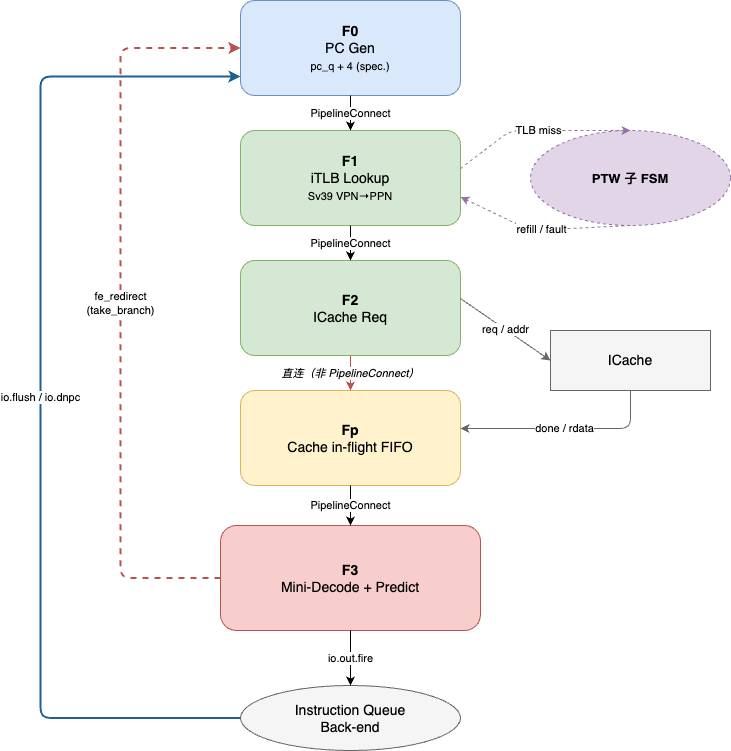
\includegraphics{ifu-pipeline.png}
  \caption{4 段流水化 IFU 的整体架构}
  \label{fig:ifu-pipeline}
\end{figure}

除 F2 $\to$ Fp 这一路外，其余子模块均通过 \lstinline|PipelineConnect| 串联。\lstinline|PipelineConnect| 本质上是一个参数化流水级：它在上下游之间插入带握手的 valid 寄存器和 \lstinline|bits| 锁存寄存器；当 \lstinline|thisIn.ready| 为高时，接收上一拍的 \lstinline|prevOut.valid / bits|；当 \lstinline|flush| 有效时，清零 valid 并丢弃当前槽位。稳态下，流水按 \lstinline|ready / valid| 协议持续推进；发生 \lstinline|flush| 时，可在同一拍清空所有中间 slot。实现上通过 Scala 泛型参数 \lstinline|T <: Data| 抽象载荷类型，使其既能承载 IFU 内部的 \lstinline|F1In|、\lstinline|F2In|、\lstinline|F3In| 等 Bundle，也能复用于后端分派、发射与执行阶段，从而保持全项目流水接口风格一致：

\begin{lstlisting}[language=Scala,caption={参数化流水段 PipelineConnect 的实现},label={lst:pipeline-connect}]
object PipelineConnect {
  def apply[T <: Data](
      prevOut: DecoupledIO[T],
      thisIn:  DecoupledIO[T],
      flush:   Bool
  ): Unit = {
    val valid = RegInit(false.B)
    when(flush) {
      valid := false.B
    }.elsewhen(thisIn.ready) {
      valid := prevOut.valid
    }
    prevOut.ready := thisIn.ready
    thisIn.bits
      := RegEnable(prevOut.bits, prevOut.valid && thisIn.ready)
    thisIn.valid  := valid
  }
}
\end{lstlisting}

F0 位于 IFU 顶层，不作为独立子模块存在，只维护架构 PC 寄存器 \lstinline|pc_q|。在每个周期，F0 都投机地按 \lstinline|pc_q + 4| 推进到 F1。若 F3 确认出现 taken 分支（如直接跳转、被预测为跳转的条件分支等），前端会立即执行自重定向，将 \lstinline|pc_q| 拉回预测目标。除此之外，凡是需要改写 PC 的情况（分支误预测、trap、xret、\lstinline|fence.i|、\lstinline|sfence.vma|、CSR 写等），统一由后端通过 \lstinline|io.flush| 携带正确的 \lstinline|io.dnpc| 来重写 \lstinline|pc_q|。顶层还会生成全局 squash 信号 \lstinline!squash = fe_take_branch | io.flush!，并广播到所有 \lstinline|PipelineConnect| 的 \lstinline|flush| 端口，以及 F1 与 Fp 的内部状态寄存器，从而保证整条流水在同一拍内同步清空。F1、F2+Fp、F3 三段的具体实现见下文。

\subsection{F1 级：MMU 地址翻译}\label{sec:ifu-mmu}

F1 承担取指侧的地址翻译职责，是前端事实上的 MMU 级，其典型实现即本文的 \lstinline|F1Stage| 子模块。模块内部由一个 16 项全相联的 iTLB 与一个 PTW 子 FSM 组成：iTLB 负责命中时的快路径，PTW 负责缺失时的慢路径回填；iTLB 的替换策略采用位矩阵 LRU（Bit-Matrix LRU）算法~\cite{belady1966replacement}，详见~\ref{sec:tlb} 节。Sv39 未启用时 F1 直接将虚拟地址低位截断作为物理地址组合放行；启用后则对 PC 的 VPN 做一次组合查表，命中且 PTE.X 合法（该页可执行）则一拍内输出翻译后的物理地址，命中但 PTE.X 不合法则置位 \lstinline|page_fault| 标志并向 F2 输出 mcause = 12 的指令页错误；若 TLB 缺失，则启动 PTW 沿 \lstinline|ptw_port| 走三级页表，完成后回填 iTLB 并在下一拍重查。

PTW 子 FSM 是整个 F1 中唯一的状态机，需要与后文~\ref{sec:ptw} 节的 PTW 内部九态遍历 FSM 区分：前者是 F1Stage 内部用于驱动 PTW 请求/响应握手并与上层 squash 协同的外层 FSM，后者才是真正执行三级页表遍历的内部算法状态机。该外层 FSM 的主路径为 \lstinline|idle -> req -> waitResp -> idle|，并在此基础上补充 squash 处理。为此，F1 维护了图~\ref{fig:ifu-ptw-fsm} 所示的四状态握手 FSM，并配合两个辅助寄存器 \lstinline|ptw_vpn_reg| 与 \lstinline|ptw_abandoned| 记录在途请求上下文。

\begin{figure}[H]
  \centering
  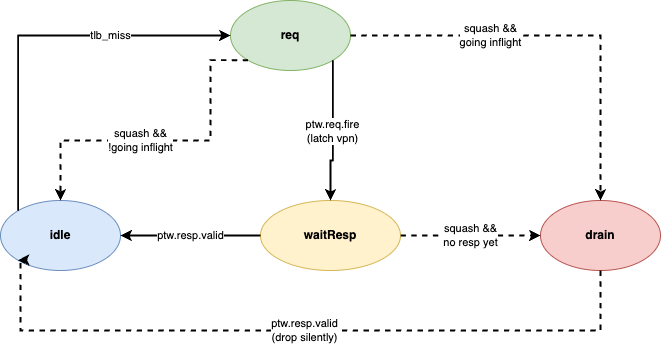
\includegraphics{ifu-ptw-fsm.png}
  \caption{F1 内部 PTW 子 FSM 状态转移图（虚线表示 squash 路径）}
  \label{fig:ifu-ptw-fsm}
\end{figure}

先看正常路径：\lstinline|idle -> req -> waitResp -> idle|。在 \lstinline|idle| 检测到 \lstinline|tlb_miss| 后，FSM 进入 \lstinline|req|，等待 PTW 接收新事务；当 \lstinline|ptw.req.fire| 成功握手后，将当前 VPN 锁存到 \lstinline|ptw_vpn_reg|，并转入 \lstinline|waitResp|；当页表遍历完成（\lstinline|ptw.resp.valid| 到达后），FSM 回到 \lstinline|idle|。此时只有同时满足“未被放弃（\lstinline|!ptw_abandoned|）、无 fault、F1 当前仍持有同一 VPN（\lstinline|in_vpn === ptw_vpn_reg|）”三条条件，才会真正 refill iTLB；否则将该响应视为过期并静默丢弃，避免错误 PPN 写入 iTLB。

再看 squash 路径（图~\ref{fig:ifu-ptw-fsm} 中虚线）。若 squash 发生时总线上已有在途页表读请求（例如 \lstinline|req| 已握手成功，或已进入 \lstinline|waitResp| 但响应尚未返回），则置 \lstinline|ptw_abandoned = 1| 并转入 \lstinline|drain|，后续仅静默吞掉响应，不 refill、也不报告 fault。其余情况下（如 \lstinline|req| 尚未握手，或 \lstinline|waitResp| 与响应同拍到达），说明不存在未决事务，可直接回到 \lstinline|idle|。\lstinline|drain| 本质上是纯等待态：一旦收到响应即返回 \lstinline|idle|。

\subsection{F2 + Fp 级：ICache 控制}\label{sec:ifu-icache-ctrl}

F2 与 Fp 在实现上对应 \lstinline|F2Stage|、\lstinline|FpStage| 两个子模块，但在功能上共同构成“ICache 控制级”：F2 负责发请求，Fp 负责跟踪响应。其中 F2 $\to$ Fp 是整条 IFU 中唯一不使用 \lstinline|PipelineConnect| 的通路。

F2 是纯组合段，不持有寄存器。它根据 \lstinline|F2In| 驱动 \lstinline|icache.req / addr / size| 并完成 \lstinline|req / ack| 握手；地址按 \lstinline|dataBytesBits| 对齐，请求仅在“上游有效、非 fault、且 Fp 有空槽”时发起，避免无效占用 ICache 带宽。对 F1 上报的 page fault，F2 走 fault bypass 直送 F3、绕过 Fp（故障表项不应占用 inflight 槽位）。cache 路径与 fault 路径最终由 fault 优先 Mux 汇合为同一份 \lstinline|F3In|，再经 \lstinline|PipelineConnect| 进入 F3。

Fp 是 IFU 中承载多条 inflight cache 读的核心结构，实现为深度 4 的环形 FIFO。采用 4 深度而非单项缓冲，是为了匹配 ICache 连续命中时“每拍可接收新请求”的流水能力，避免 F2 过早反压。Fp 使用三个指针：\lstinline|enq_ptr|（F2 入队）、\lstinline|deq_ptr|（F3 出队）和 \lstinline|rdata_ptr|（响应回填）；前两者通过翻转位区分满/空，\lstinline|rdata_ptr| 在每次 \lstinline|icache.done| 时写入 \lstinline|slots(rdata_ptr)|。

Fp 的 squash 策略比 F1 更直接：\lstinline|squash = 1| 同拍复位三个指针。此后即使旧响应返回，也会因 \lstinline|!has_inflight| 被忽略，不再写入槽位。

\subsection{F3 级：预测与后端交付}

F3（\lstinline|F3Stage|）是整条 IFU 的交付点。结构上，F3 本身是纯组合逻辑，唯一的时序元件来自其输入侧 \lstinline|PipelineConnect| 持有的 slot 寄存器。F3 的职责主要有三项：切出指令字、驱动 Predict 端口、生成前端自重定向脉冲。

若上游表项已标记 \lstinline|has_fault|，则 F3 强制将指令字置 0，并在 \lstinline|IFUOutput| 中输出 \lstinline|mcause = 12|、\lstinline|mtval = pc|、\lstinline|has_except = 1|，供后端在 ROB 提交点统一触发 trap。

Predict 端口以 \lstinline|pc|、\lstinline|inst| 为输入，以 \lstinline|dnpc|、\lstinline|ghr|(global history register) 为输出；F3 在同一拍将预测结果与原始指令一起封装到 \lstinline|IFUOutput|。

F3 对控制冒险的收敛通过 \lstinline|fe_take_branch| 信号实现，其定义为：

\[
\mathrm{fe\_take\_branch} = (\neg\,\mathrm{has\_fault}) \wedge (\mathrm{predict.dnpc} \neq \mathrm{pc} + 4)
\]

即“F3 成功向后端交付了一条非故障指令，且预测下一 PC 不等于顺序后继 \lstinline|pc + 4|”。其对 F0 及各级 slot 的回卷影响将在下一节展开。

\subsection{推测性控制冒险与前端自重定向}\label{sec:ifu-redirect}

前端自重定向首先是在解决一个时序矛盾：\lstinline|pc_q| 必须先进入 F1 才能完成虚实地址转换，随后经 F2+Fp 才能取回指令，而分支是否跳转要到 F3 译码并调用 Predict 后才能确定。也就是说，当 F3 才知道“应当跳转”时，错误路径上的指令往往已经进入 F1/Fp 的流水；若不立即失效，这些指令就可能继续流入后端，造成错误执行。

为此，F3 额外提供一条基于预测结果的前端收敛通道 \lstinline|fe_take_branch|。当该脉冲有效时，顶层同拍执行两件事：一是广播 \lstinline|squash| 到所有 \lstinline|PipelineConnect| 以及 F1/Fp 内部状态寄存器，使在途项指令失效；二是将 \lstinline|pc_q| 从默认的 \lstinline|pc_q + 4| 改写为 \lstinline|io.predict.dnpc|，使下一拍 F0 直接从预测目标重新取指。这样，控制冒险不必等待后端回写权威 PC，即可在前端就地止损，将 taken 分支的气泡压缩到 2 拍。

这里的“推测性”在于：这次回卷只依赖前端预测。若预测错误，后端在若干拍后发现 \lstinline|redirect.dnpc| 与 \lstinline|predict_npc| 不一致，再由 CommitStage 发出 \lstinline|io.flush|，用权威 \lstinline|io.dnpc| 修正 \lstinline|pc_q|。在实现上，\lstinline|pc_q| 的更新采用优先多路复用，优先级为“后端权威 PC > 前端预测 PC > 顺序推进(PC+4)”。

同理，前端不为这类会影响 PC 的 serializing 指令（如修改 \lstinline|mtvec|/\lstinline|mepc|、\lstinline|xret|、\lstinline|ecall|、\lstinline|ebreak|）建立独立预测通道。主要矛盾在于：这些指令的下一 PC 依赖后端执行结果，前端无法在 F3 提前给出可靠预测；在实现上等价于先按顺序路径 \lstinline|pc + 4| 推进，随后由后端在检测到真实控制流后发出 \lstinline|io.flush| 进行纠正。该策略虽会引入额外回卷，但在此类指令出现频率较低、专用硬件收益有限（Amdahl 定律~\cite{amdahl1967validity}）的前提下，仍是复杂度与收益更平衡的选择。

\section{动态分支预测单元设计}\label{sec:predict}

分支预测单元（Predict）对 IFU 取到的指令进行轻量译码，复用后端的 CU（Control Unit，控制单元）与 IGU（Immediate Generate Unit，立即数生成单元）模块提取指令类型与立即数。CU 本身是后端译码级的核心模块，包含完整的指令解码逻辑，具有一定的复杂性。前端复用 CU 时，将前端不涉及的输入信号硬编码为 0，不需要的输出信号悬空；综合工具在优化阶段可据此自动裁剪不可达的组合逻辑路径，使前端实例化的 CU 仅保留指令类型识别等轻量子集，在避免重复编写译码逻辑的同时不引入多余的面积开销。Predict 根据 CU 输出的指令类型将当前指令分派到不同的预测器，最终通过优先级选择逻辑输出预测的下一条 PC。

\subsection{GShare 分支方向预测器（BHT, Branch History Table）}

对于条件分支指令，采用 GShare 算法~\cite{mcfarling1993combining} 进行方向预测。GShare 使用全局历史寄存器（GHR, Global History Register）与 PC 的高 60 位（\lstinline|PC[63:4]|）进行异或得到哈希结果，再取索引位定位模式历史表（PHT, Pattern History Table），以利用全局分支相关性提高预测精度。PHT 包含 4096 个表项，每个表项使用 2 位饱和计数器：计数器高位为 1 表示预测跳转，为 0 表示预测不跳转。当 PHT 中对应表项尚未被训练（occupied 标志为假）时，退化为静态预测——以立即数符号位作为预测方向（负偏移预测跳转，正偏移预测不跳转），该启发式对循环结构有较好的覆盖。

后端在条件分支指令提交时，通过 redirect 信号将实际跳转结果与该指令对应的 GHR 快照回传给 BHT，BHT 使用回传的 GHR 与 PC 异或重新定位 PHT 表项并更新饱和计数器，同时将实际跳转方向移入 GHR。

\begin{figure}[H]
  \centering
  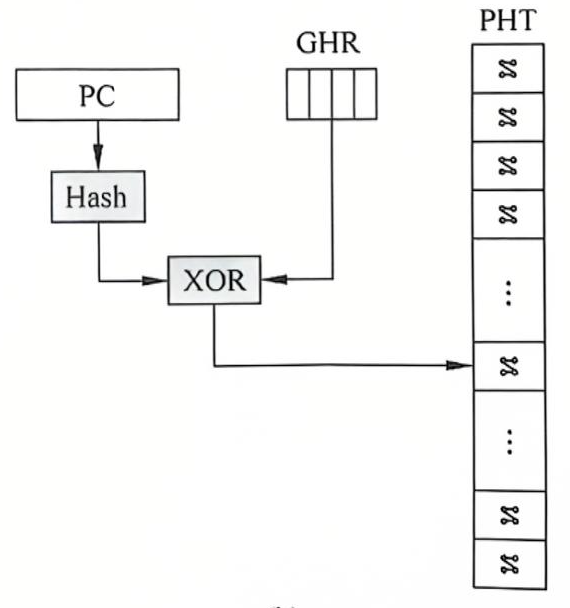
\includegraphics[width=0.45\textwidth]{gshare-xor.png}
  \caption{GShare 中 GHR 与 PC 异或索引示意}
  \label{fig:gshare-xor}
\end{figure}

\subsection{间接跳转目标缓存（IJTC, Indirect Jump Target Cache）}

对于非返回类的间接跳转指令（JALR 且非 ret 模式），采用 IJTC 进行目标地址预测。IJTC 使用 8 项全相联内容可寻址存储器（CAM, Content Addressable Memory）结构，以 PC 作为 tag 进行匹配查询。命中时直接返回缓存的目标地址；缺失时不做预测，前端将使用顺序 PC。

更新策略上，后端在 JALR 指令提交时将实际 PC 与目标地址回传给 IJTC。若 CAM 中已存在该 PC 对应的表项则原地更新目标地址；若不存在则以先进先出（FIFO, First In First Out）策略淘汰最旧表项并写入新映射。

\subsection{返回地址栈（RAS, Return Address Stack）}

对于函数返回指令，采用 RAS 进行目标地址预测。RAS 为深度 8 的循环栈，通过 rd 和 rs1 字段识别 call/ret 模式：当指令为 JAL 或 JALR 且目的寄存器为 x1 或 x5 时判定为 call，将顺序 PC（snpc = pc + 4）压栈；当指令为 JALR 且 rd = x0、rs1 = x1 时判定为 ret，弹栈并将栈顶值作为预测目标。

\begin{figure}[H]
  \centering
  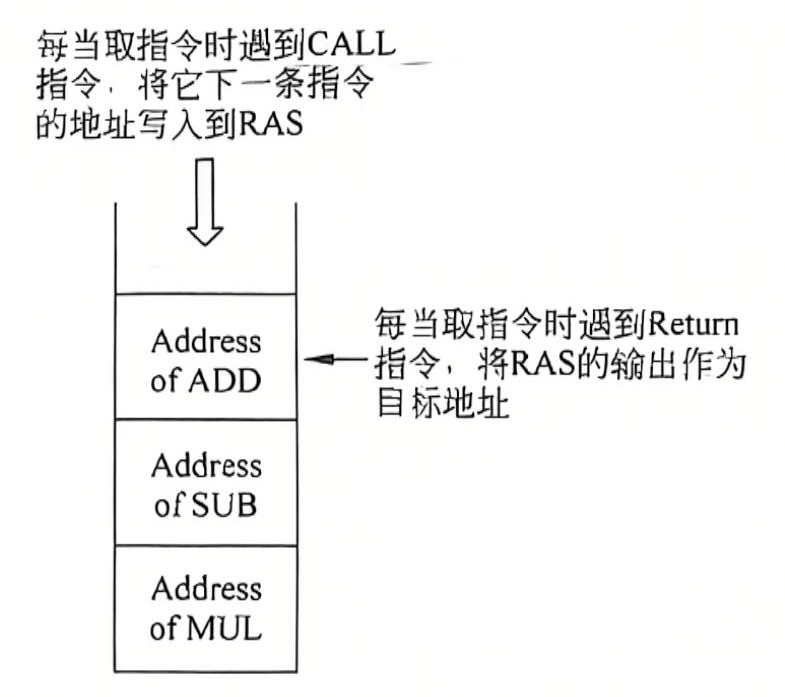
\includegraphics[width=0.5\textwidth]{ras-stack.png}
  \caption{返回地址栈（RAS）工作示意}
  \label{fig:ras-stack}
\end{figure}

\subsection{预测选择逻辑}

Predict 模块根据指令类型按优先级选择预测结果：JAL 指令直接使用 PC + 立即数作为目标；条件分支指令根据 BHT 预测方向选择跳转目标或顺序 PC；JALR 且为 ret 模式时使用 RAS 弹栈结果；JALR 且 IJTC 命中时使用 IJTC 缓存的目标地址；其余情况使用顺序 PC。预测结果与当前 GHR 快照一并传递给 IFU，由 IFU 在下一周期使用该地址取指，并随指令一同送入后端，供后端在提交时进行验证与预测器更新。

\subsection{与 BTB 方案的对比及设计取舍}

经典分支预测方案~\cite{yao2014superscalar} 通常使用分支目标缓冲器（BTB, Branch Target Buffer）：在取指阶段以 PC 索引 BTB，若命中则直接读出缓存的跳转目标地址，从而在译码之前就完成预测。BTB 的优势在于无需等待指令译码即可获得目标地址，适合流水化取指前端。

本课题的设计目标是在尽可能简单的前端实现下取得合理的预测覆盖。在本文的 4 段流水前端（\ref{sec:ifu-pipeline} 节）中，预测器工作在 F3 阶段——指令字已在 F3 可见，指令类型与立即数可得。对于 JAL 和 BRANCH 这两类指令，目标地址为 PC + 立即数的简单加法，可在当拍直接计算得出，无需额外的缓存结构；仅对 JALR 这类目标地址依赖寄存器值、前端无法计算的指令，才借助 IJTC 或 RAS 进行预测。因此在本微架构下，BTB 的作用被直接计算和专用预测器所替代，省去了 BTB 的存储开销与维护逻辑；后续若进一步优化时序，拆分取指流水线，则 BTB 才会成为必要的补充。

\subsection{预测器更新策略}

三个预测器的更新策略根据各自特性采用了不同的时机。

GShare 与 IJTC 采用保守策略，仅在指令提交（commit）时更新。后端通过 redirect 信号将已提交的分支指令的实际跳转结果、PC 与 GHR 快照回传给前端预测器。这一策略的优势在于只有确认正确执行路径上的指令才会影响预测器状态，避免了因推测执行路径上的错误信息污染 PHT 或 IJTC 表项。

RAS 则采用激进策略，在前端取指与预解码阶段即时更新：遇到 call 指令立即压栈，遇到 ret 指令立即弹栈。这一设计是合理的——即使当前指令处于推测路径上，推测路径中的 call 与 ret 仍然是成对出现的，压栈与弹栈操作相互抵消，不会破坏栈的正确性。若在前端就更新 RAS，后续紧跟的 ret 指令可以立即获得正确的返回地址，而无需等待 call 指令提交，从而降低了函数调用密集场景下的预测延迟。

\section{本章小结}

本章围绕“前端取指流水化、分支预测”两条主线介绍了 IFU 与动态分支预测的设计。

在取指流水化方面，IFU 采用 F0、F1、F2、Fp、F3 的流水结构，以“直线代码稳态 1 IPC、taken 分支仅引入 2 拍气泡”为性能目标。F1 作为 MMU 级完成 iTLB 查询与 PTW 慢路径遍历；F2 与 Fp 共同构成 ICache 控制级，F2 负责请求通道、Fp 以深度 4 的环形 FIFO 追踪在飞响应，二者间以直连代替 \lstinline|PipelineConnect| 以满足 ICache 握手时序；F3 作为提交点在一拍内完成指令切分、预测驱动与后端交付。

在分支预测方面，设计采用 GShare + IJTC + RAS 的组合方案，分别对应条件分支、间接跳转与函数返回三类控制流。得益于前端已完成预解码，JAL 与 BRANCH 的目标地址可直接由 PC 与立即数相加得到，仅 JALR 需借助专用预测器，从而省去了 BTB 的存储与维护开销。更新策略上，GShare 与 IJTC 采用提交时更新的保守策略以避免推测路径污染预测器状态；RAS 则在进入后端指令队列当拍完成 push/pop，借助 call/ret 的成对性降低返回预测延迟。

在推测性控制冒险处理上，前端通过 F3 的 \lstinline|fe_take_branch| 脉冲就地收敛 taken 分支，将气泡压缩到 2 拍。除此之外，所有需要前端回卷的场景统一交给后端 CommitStage 发出的 \lstinline|io.flush| 处理，其触发可分为以下两类：

\begin{enumerate}
  \item “改 PC”事件，包括分支误预测、trap 与 xret：后端确定权威目标后，以 \lstinline|io.flush| + \lstinline|io.dnpc| 对 \lstinline|pc_q| 做二次回卷。
  \item “影响前端状态但不一定改 PC”的事件，包括 \lstinline|fence.i|（ICache cacheline 失效）、\lstinline|sfence.vma|（iTLB 表项失效）以及改变 \lstinline|satp|/特权级的 CSR 写：即便 PC 可保持顺序，前端仍需同拍清空所有 inflight 事务，并按后端给出的 \lstinline|io.dnpc|（通常为 \lstinline|pc+4|）重新取指。
\end{enumerate}

关于分支预测命中率、前端 flush 事件分解及其与三组基准程序（MicroBench / Dhrystone / CoreMark）的分析，详见~\ref{sec:perf-fe-breakdown} 节与表~\ref{tbl:perf-bp}。

% !Mode:: "TeX:UTF-8"

\chapter{后端：乱序执行引擎}\label{sec:backend}

后端接收前端经指令队列送入的指令流，完成译码、寄存器重命名、发射、执行、写回与提交的全流程，是实现乱序执行的核心引擎~\cite{smith1995superscalar}。本文实现的后端支持 RV64IM 指令集架构，包含整数运算、乘除法运算、分支、访存与控制状态寄存器（CSR, Control and Status Register）五条执行路径。

\begin{figure}[H]
  \centering
  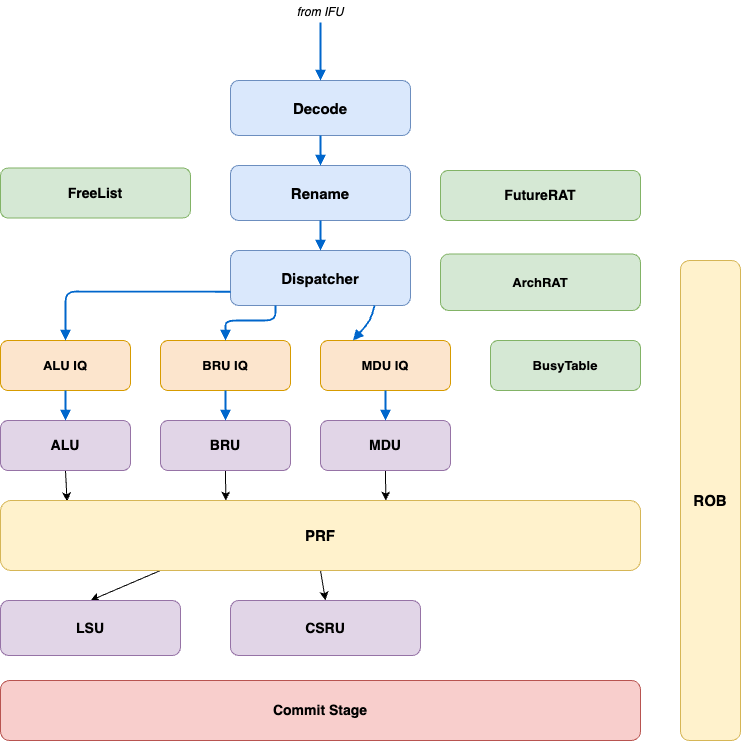
\includegraphics{backend-arch.png}
  \caption{后端乱序执行引擎（仅展示核心数据通路）}
  \label{fig:backend-arch}
\end{figure}

如图~\ref{fig:backend-arch} 所示，后端按“译码—重命名—分派—发射—执行—（延迟执行）—提交”的主路径组织。指令进入 Decode 后，在 Rename 阶段结合 FutureRAT 与 FreeList 完成物理寄存器分配，随后在 Dispatcher 一方面写入 ROB，另一方面按类型分发到 ALU IQ、BRU IQ、MDU IQ。各发射队列在满足就绪条件后驱动对应执行单元，执行结果统一写回 PRF，并由 ROB 负责跟踪完成与提交顺序。图中同时给出了 BusyTable、ArchRAT、LSU、CSRU 与 Commit Stage 在提交路径中的位置：其中 LSU/CSRU 走延迟执行路径，由 ROB 在接近提交时交付；Commit Stage 再从 ROB 头部按序提交，完成 ArchRAT 更新与 FreeList 回收，实现从乱序执行到顺序提交的状态收敛~\cite{choi2013rob}~\cite{smith1988precise}。为突出主干流程，图中省略了控制信号与回写细连线。

\section{译码级}

译码级接收前端送入的指令字与 PC，通过 CU（Control Unit）解码出指令类型、功能单元选择、操作码、源/目的寄存器编号等控制信号，通过 IGU（Immediate Generate Unit）提取并符号扩展立即数。译码级的输出形成完整的微操作描述，经流水线寄存器\footnote{该流水线寄存器采用前文 \lstinline|PipelineConnect| 实现，见代码~\ref{lst:pipeline-connect}。}传递给重命名级。

CU 的实现利用了 Chisel 提供的 \lstinline|DecodeTable| 框架与 Espresso 逻辑最小化工具~\cite{chipsalliance_espresso}。具体而言，首先定义 \lstinline|InstPattern| 作为指令编码的匹配模板，将 func7、rs2、func3、opcode 四个字段组合为 \lstinline|BitPat|，其中不相关的位标记为 don't-care：

\begin{lstlisting}[language=Scala,caption={指令匹配模板 InstPattern 定义},label={lst:inst-pattern}]
case class InstPattern(
  func7: BitPat = BitPat.dontCare(7),
  rs2:   BitPat = BitPat.dontCare(5),
  func3: BitPat = BitPat.dontCare(3),
  opcode: BitPat
) extends DecodePattern {
  def bitPat = func7 ## rs2 ## BitPat.dontCare(5)
    ## func3 ## BitPat.dontCare(5) ## opcode
}
\end{lstlisting}

随后，为每个需要译出的控制信号定义一个 \lstinline|DecodeField|，在其 \lstinline|genTable| 方法中以 Scala 模式匹配的方式描述每条指令对应的输出值。所有指令模板与译码字段汇总为一张 \lstinline|DecodeTable|，Chisel 编译期自动调用 Espresso 对真值表进行两级逻辑最小化，生成面积最优的组合逻辑电路。相比手工编写 \lstinline|MuxLookup| 或 \lstinline|switch| 译码树，该方案在指令数量增长时仍能保持紧凑的门级实现，同时 Scala 的类型系统与模式匹配语法使译码表的维护更加直观，新增指令只需在 \lstinline|allInstructions| 列表中追加一行 \lstinline|InstPattern| 并在各 \lstinline|DecodeField| 中补充对应映射即可，如代码~\ref{lst:decode-table-example} 所示。

\begin{lstlisting}[language=Scala,caption={DecodeTable 指令模板与字段汇总示例},label={lst:decode-table-example}]
val allInstructions = Seq(
  InstPattern(func7 = BitPat("b0000000"),
    func3 = BitPat("b000"),
    opcode = BitPat("b0110011")), // ADD
  ...
)

object CsrOpField extends DecodeField[InstPattern, UInt] {
  def name = "csr_op"
  def genTable(op: InstPattern) = op.opcode.rawString match {
    case OP_SYSTEM =>
      op.func3.rawString match {
        case "001" => bp(CSROpType.CSR_RW)
        case _     => dc
      }
    case _ => dc
  }
}

val allFields = Seq(
  CsrOpField,
  ...
)

val decodeTable = new DecodeTable(allInstructions, allFields)
\end{lstlisting}

CU 的译码输出涵盖 9 个字段：指令类型（\lstinline|InstType|，18 种）、ALU 操作码（\lstinline|ALUOpType|）、MDU 操作码（\lstinline|MDUOpType|）、立即数类型（\lstinline|ImmType|，I/S/B/U/J 五种）、BRU 操作码（\lstinline|BRUOpType|）、访存宽度与符号扩展标志、CSR 操作类型与写使能。对于 ECALL、EBREAK 与非法指令，CU 额外输出异常标记与 mcause/mtval 初始值，供提交级进一步处理。

\section{寄存器重命名}

寄存器重命名是乱序执行的核心前提~\cite{tomasulo1967algorithm}，其目的是消除指令间由逻辑寄存器复用导致的 WAW（写后写）与 WAR（写后读）假依赖，使真正的数据依赖（RAW）成为唯一的调度约束。本文采用统一物理寄存器文件（Unified Physical Register File, PRF）方案，主要涉及以下结构：

物理寄存器文件（PRF）。PRF 提供 9 个读端口与 5 个写端口。9 个读端口分配给 ALU（2）、BRU（2）、MDU（2）、LSU（2）与 CSRU（1）五条执行路径；5 个写端口分别服务于 ALU 写回、分派级立即数写入、LSU 写回、CSR 写回与 MDU 写回。

Future RAT(future register alias table)。Future RAT 维护推测状态下的逻辑寄存器到物理寄存器映射表。重命名级通过 3 个读端口查询源寄存器（rs1、rs2）与目的寄存器（rd）当前映射的物理寄存器号，随后从 FreeList 分配一个空闲物理寄存器作为 rd 的新映射，并将新映射写回 Future RAT。旧的 rd 映射（old\_prd）随指令一同写入 ROB，供提交时释放。

Arch RAT(architectural alias table)。Arch RAT 维护已提交的确定性映射。每当指令提交时，CommitStage 将该指令的逻辑目的寄存器与新物理寄存器映射写入 Arch RAT，并将 old\_prd 归还 FreeList。Arch RAT 始终反映最近一次已提交指令的寄存器状态。

FreeList。FreeList 管理空闲物理寄存器池。重命名级从中分配新物理寄存器，提交级向其归还不再需要的物理寄存器。归还的依据是：当一个逻辑寄存器被后续指令重新定义（即发生 WAW）时，承载旧值的物理寄存器的生命周期随之结束，可以被安全释放。以如下指令序列为例：

\begin{table}[H]
  \centering
  \caption{重命名分配示例}
  \label{tbl:rename-example}
  \begin{tabular}{cccc}
    \toprule
    指令 & 逻辑 rd & 分配 prd & old\_prd \\
    \midrule
    ADD x1, x2, x3 & x1 & p10 & p1 \\
    SUB x1, x4, x5 & x1 & p11 & p10 \\
    \bottomrule
  \end{tabular}
\end{table}

ADD 将 x1 的映射从 p1 更新为 p10，此时 p1 成为 old\_prd。当 ADD 提交时，p1 承载的旧值已无任何指令需要读取（后续所有引用 x1 的指令都将读到 p10 或更新的映射），因此 p1 可以归还 FreeList。同理，当 SUB 提交时，x1 的映射再次更新为 p11，p10 的生命周期结束并被归还。通过这一机制，物理寄存器的分配与回收严格跟随逻辑寄存器的定义链，保证了在任意时刻每个“活跃值”都独占一个物理寄存器，不会出现数据覆盖。当发生 flush 时，FreeList 根据 Arch RAT 快照重建：凡不在 Arch RAT 映射中的物理寄存器均标记为空闲，一拍即可完成恢复。

BusyTable。BusyTable 记录每个物理寄存器的数据就绪状态。重命名级在分配新物理寄存器时将其标记为 busy；当结果产生时通过 wakeup 信号清除 busy 标记。发射队列在发射前查询 BusyTable 以判断源操作数是否就绪。BusyTable 配置 6 个读端口供三个发射队列使用（每队列 2 个，对应 rs1 和 rs2），5 个 wakeup 端口对应三类时机：（1）分派级即时唤醒——LUI、AUIPC、JAL、JALR 等指令的结果仅依赖 PC 与立即数，在分派级即可计算并写入 PRF，同时发出 wakeup；（2）执行完毕唤醒——ALU 与 MDU 执行单元写回结果时发出 wakeup；（3）延迟执行完毕唤醒——LSU 与 CSRU 在 ROB 调度下完成延迟执行并写回 PRF 后发出 wakeup。三类唤醒覆盖了指令生命周期中所有可能产生结果的阶段，使后续依赖指令能尽早感知操作数就绪并被发射。

Flush 恢复机制。当后端检测到分支预测错误或异常时，flush 信号同时送往 ROB、FreeList、BusyTable、FutureRAT 以及所有发射队列。FutureRAT 从 Arch RAT 的快照一拍恢复到已提交状态的映射；FreeList 同样根据 Arch RAT 快照重建空闲池。由于 Arch RAT 在提交时同步更新，其内容始终正确，因此恢复过程无需遍历 ROB，仅需一个周期。

\section{分派级}

分派级位于重命名级之后，负责将已完成寄存器重命名的微操作分发到对应的执行资源。分派级执行以下操作：

\begin{enumerate}
  \item 将指令写入 ROB，获取 ROB 标签（rob\_tag）作为指令在乱序流水线中的唯一标识。
  \item 根据指令类型将指令分派到对应的发射队列：ALU 类指令进入 ALU IQ、乘除法指令进入 MDU IQ、 分支指令进入 BRU IQ。
  \item 对于结果可在分派级直接确定的指令——JAL、JALR、LUI 与 AUIPC——分派级直接将计算结果写入 PRF 并发出 wakeup 信号，无需经过执行单元。这些指令的结果（链接地址 pc+4 或立即数加载值）仅依赖 PC 与立即数，在译码后即可获得，提前写回可减少后续依赖指令的等待周期。
  \item 对于访存指令与 CSR 指令，采用保守的延迟执行策略：分派级仅将其写入 ROB，不送入发射队列，待指令到达 ROB 提交头部时再交由 LSU 或 CSRU 执行。访存指令的延迟执行避免了推测路径上的 Store 对内存状态造成不可撤销的副作用，简化了存储一致性维护；CSR 指令的延迟执行保证了特权级切换、中断使能等副作用严格按程序顺序生效，防止推测执行引发错误的系统状态变更。
\end{enumerate}

\section{发射队列与乱序发射}

后端设置三个独立的发射队列，分别服务于 ALU、MDU 和 BRU 执行单元。在实现层面，得益于 Chisel 作为 Scala 嵌入式 DSL 的语言特性，发射队列采用泛型抽象类设计：

\begin{lstlisting}[language=Scala,caption={泛型发射队列抽象类定义},label={lst:issue-queue-abs}]
abstract class IssueQueue[T <: Data]
  (gen: T, val entries: Int)
  extends NPCModule {
    ...
  }
\end{lstlisting}

三个发射队列共享相同的入队、就绪检测与发射选择逻辑，唯一的差异在于类型参数 \lstinline|gen| 所携带的附加数据——例如 ALU 发射队列的 \lstinline|gen| 包含立即数与 ALU 操作码字段，而 BRU 和 MDU 的 \lstinline|gen| 则不含立即数。通过 Scala 的参数化类型，三个队列复用同一套核心实现，仅在类型层面区分载荷内容，避免了重复代码。同时，\lstinline|abstract class| 的设计允许派生出不同复杂度的具体实现：简单实现采用固定槽位逐项扫描，复杂实现可引入压缩表项（compacting entry）以在指令发射后自动前移后续表项、提高槽位利用率，两者对外接口完全一致，便于在面积与时序之间灵活权衡。

每个发射队列在入队时记录指令的源物理寄存器号与 ROB 标签，在发射前通过 BusyTable 的读端口查询两个源操作数的就绪状态。当源操作数全部就绪时，指令即可被选中发射。由于多条指令可能同时就绪，发射队列内部通过优先级编码器选择最早入队的指令发射，保证公平性。

wakeup 机制是乱序发射的关键驱动力。后端共有 5 个 wakeup 源：ALU 写回、MDU 写回、分派级立即数写入、LSU 写回与 CSRU 写回。当任一执行路径产生结果时，对应的 wakeup 信号广播到 BusyTable，将目的物理寄存器标记为就绪。发射队列在下一周期即可感知新的就绪状态并发射等待该操作数的指令，形成“执行—唤醒—发射”的连锁反应。

\section{执行单元}

后端包含五条执行路径，各路径独立运行，互不阻塞。与发射队列的设计思路类似，执行单元同样抽象出统一的泛型接口：

\begin{lstlisting}[language=Scala,caption={执行单元抽象基类定义},label={lst:exec-unit-abs}]
abstract class ExecUnit[I <: Data, O <: Data](
  inGen: I, outGen: O, numReadPorts: Int = 2
) extends NPCModule {
  val prs1 = IO(Input(UInt(NRPhyRegBits.W)))
  val prs2 = IO(Input(UInt(NRPhyRegBits.W)))
  val prf  = IO(Vec(numReadPorts, new PRFReadPort))
  val io = IO(new Bundle {
    val in  = Flipped(Decoupled(inGen))
    val out = Decoupled(outGen)
  })
}
\end{lstlisting}

\lstinline|ExecUnit| 通过类型参数 \lstinline|I| 和 \lstinline|O| 分别参数化输入载荷与输出载荷，所有执行单元共享统一的 PRF 读端口接口（\lstinline|prs1|、\lstinline|prs2|、\lstinline|prf|）与 Decoupled 握手协议（\lstinline|io.in| / \lstinline|io.out|）。ALU、MDU 与 BRU 继承该抽象类并特化各自的输入输出类型：ALU 的输入包含 ALU 操作码、立即数与立即数选择标志，输出包含运算结果与目的物理寄存器号；MDU 的输入包含 MDU 操作码，输出结构与 ALU 相同；BRU 的输入仅包含分支操作码，输出为分支结果标志（br\_flag）。这一设计使后端连线层可以统一处理发射队列到执行单元的对接逻辑，同时各执行单元内部实现完全独立。

ALU 路径。处理整数算术逻辑运算（加减、移位、比较、逻辑运算等）。ALU 为单周期执行，从 ALU IQ 发射后经 PRF 读取源操作数、执行运算、写回 PRF 并向 ROB 报告完成，同时发出 wakeup。

MDU 路径。处理乘法与除法运算。MDU 执行延迟不固定（乘法与除法周期数不同），通过 valid/ready 握手协议与发射队列和 ROB 交互。写回逻辑与 ALU 路径相同。

BRU 路径。处理条件分支指令的实际比较。BRU 从 BRU IQ 发射后读取源操作数并计算分支条件（br\_flag），将结果报告给 ROB。BRU 不写 PRF——条件分支指令无目的寄存器。

\section{延迟执行单元}\label{sec:late-exec}

与通过发射队列乱序发射的 ALU/MDU/BRU 不同，LSU 与 CSRU 采用延迟执行（late execution）模式：指令在分派时仅写入 ROB，待到达 ROB 提交头部时才交付执行。延迟执行单元同样抽象出统一的泛型基类：

\begin{lstlisting}[language=Scala,caption={延迟执行单元抽象基类定义},label={lst:late-exec-abs}]
abstract class LateExecUnit[T <: Data](
  gen: => T, numReadPorts: Int
) extends NPCModule {
  val late = IO(Flipped(ReqDone(gen)))
  val prf  = IO(Vec(numReadPorts, new PRFReadPort))
}
\end{lstlisting}

\lstinline|LateExecUnit| 通过类型参数 \lstinline|T| 参数化 ROB 传入的请求载荷，\lstinline|late| 端口采用 \lstinline|ReqDone| 握手协议（ROB 发起请求、执行单元返回完成），\lstinline|prf| 提供 PRF 读端口用于读取源操作数。LSU 与 CSRU 继承该基类并特化各自的请求类型与读端口数量。

LSU 路径。处理 Load/Store 指令。ROB 将访存指令送至提交头部后通过 \lstinline|late| 端口交给 LSU，确保访存操作按程序顺序执行，简化了存储一致性维护。LSU 内部连接 DCache 与外设端口，并集成 dTLB 与 PTW 以支持 Sv39 地址翻译。LSU 写回通过独立的 PRF 写端口与 wakeup 通路完成。

CSRU 路径。处理 CSR 读写指令。与 LSU 类似，由 ROB 在提交阶段通过 \lstinline|late| 端口交给 CSRU 执行，保证 CSR 操作的顺序语义。CSRU 同时负责中断与异常的状态管理，包括 trap 入口计算、mret/sret 返回地址提供、中断挂起检测等。

\section{提交级}

提交级（CommitStage）从 ROB 头部按程序顺序逐条提交指令，是乱序执行恢复顺序语义的关键环节。提交时执行以下操作：

(1) 将指令的目的逻辑寄存器与新物理寄存器映射写入 Arch RAT，使确定性状态前进。

(2) 将旧物理寄存器号（old\_prd）归还 FreeList，供后续指令重命名时分配。

(3) 检查异常与中断：若提交头部的指令携带异常标记（如 page fault、非法指令）或检测到中断挂起，CommitStage 触发 trap 流程，通过 CSRU 获取 trap 入口地址，生成 redirect 信号指向异常处理程序，并发出 flush 清空流水线。

(4) 处理 mret/sret 返回：提交 mret 或 sret 指令时，从 CSRU 读取 mepc 或 sepc 作为 redirect 目标。

(5) 处理 fence.i 与 sfence.vma：提交这两类指令时，分别向外输出 fence\_i 和 sfence\_vma 信号，通知 ICache 失效或 TLB 刷新。

(6) 分支验证：对于条件分支指令，将 BRU 写回的实际跳转结果与前端预测进行比对。若预测错误，生成 redirect 信号携带正确的目标地址与分支信息，同时发出 flush。

(7) 调试探针（probe）：提交时输出指令的 PC、下一条 PC、指令字、通用寄存器（GPR, General Purpose Register）状态与 CSR 状态等信息，供 DiffTest 框架与参考模型逐条比对，实现运行时正确性验证。

\section{本章小结}

本章介绍了后端乱序执行引擎的设计。后端采用译码、重命名、分派、发射、执行、写回、（晚执行）、提交的经典乱序流水线结构，通过统一物理寄存器文件与 FutureRAT/ArchRAT 双映射表实现寄存器重命名，消除 WAW 与 WAR 假依赖。五条独立执行路径（ALU、MDU、BRU、LSU、CSRU）并行运行，其中 ALU/MDU/BRU 通过发射队列乱序发射，LSU 与 CSRU 通过 ROB 延迟执行以保证顺序语义。提交级按序提交并处理异常、中断、分支验证与调试输出。flush 恢复仅需一周期，利用 ArchRAT 快照同时重建 FutureRAT 与 FreeList。

% !Mode:: "TeX:UTF-8"

\chapter{RISC-V 特权级架构}

本章介绍处理器的特权级架构、精确异常与中断机制的设计与实现。实现主要参考 RISC-V 特权级规范~\cite{riscv2024priv}、监督二进制接口（SBI, Supervisor Binary Interface）规范~\cite{riscv2024sbi} 以及 PLIC~\cite{riscv2024plic} 与 CLINT 规范手册~\cite{sifive2024interrupt}。

\section{M/S/U 三级特权架构}

处理器实现了 RISC-V 规范定义的三级特权模式：M-mode（机器模式）、S-mode（监管模式）与 U-mode（用户模式）。当前特权级由 CSRU 内部的 \lstinline|priv| 寄存器维护，上电复位后初始化为 M-mode。特权级的切换由两类事件驱动：

\begin{enumerate}
  \item 陷入（Trap）：异常或中断发生时，处理器根据委托寄存器（medeleg/mideleg）决定陷入到 M-mode 还是 S-mode，并将当前特权级保存到 mstatus 的 MPP 或 SPP 字段。
  \item 返回（xRET）：执行 mret 时从 mstatus.MPP 恢复特权级；执行 sret 时从 mstatus.SPP 恢复特权级。
\end{enumerate}

图~\ref{fig:priv-fsm} 展示了 M/S/U 三级特权模式之间的完整转换关系。

\begin{figure}[H]
  \centering
  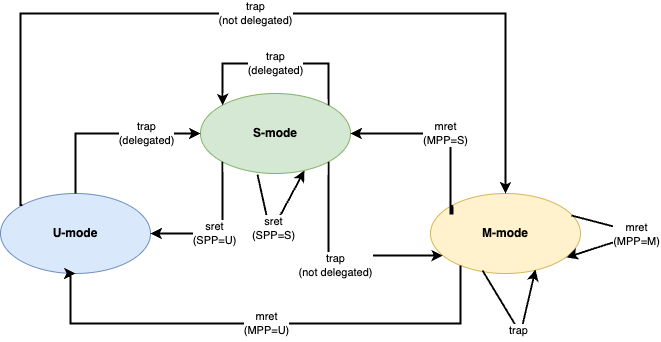
\includegraphics{priv-fsm.png}
  \caption{M/S/U 特权级状态机}
  \label{fig:priv-fsm}
\end{figure}

通过委托(delegate)机制，操作系统可在 S-mode 直接处理用户态的系统调用与页错误等常见异常，无需经过 M-mode 中转，降低了 trap 延迟。常见的操作系统，如 Linux, NetBSD 等，均运行在 S-mode 并且开启委托机制。

\section{CSR 寄存器文件}

CSRU 内部实现了完整的 M-mode 与 S-mode CSR 寄存器集合：

\begin{table}[H]
  \centering
  \caption{CSR 寄存器集合}
  \label{tbl:csr-set}
  \begin{tabular}{cll}
    \toprule
    模式 & 寄存器 & 功能 \\
    \midrule
    M & mstatus, mtvec, mepc, mcause, mtval & 状态、陷入入口、异常现场 \\
    M & medeleg, mideleg & 异常/中断委托 \\
    M & mie, mip & 中断使能与挂起 \\
    M & mscratch, menvcfg, mcounteren & 暂存、环境配置、计数器访问 \\
    M & pmpcfg0, pmpaddr0 & 物理内存保护 \\
    M & mvendorid, marchid, mhartid, misa & 只读标识（RV64IMASU） \\
    S & sstatus, stvec, sepc, scause, stval & S-mode 状态与陷入现场 \\
    S & sie, sip, sscratch, satp & 中断使能、暂存、页表基址 \\
    S & stimecmp & S-mode 定时器比较值 \\
    \bottomrule
  \end{tabular}
\end{table}

其中 sstatus、sie 与 sip 并非独立寄存器，而是 mstatus、mie 与 mip 的掩码视图（masked view）。例如 sstatus 的读取值为 \lstinline|mstatus & SSTATUS_MASK|，写入时仅修改掩码对应位，其余位保持不变。这一设计与 RISC-V 规范一致，避免了 M/S 两级寄存器状态的冗余与不一致。

CSR 指令支持三种操作类型：CSRRW（读后写）、CSRRS（读后置位）与 CSRRC（读后清零），写入数据分别为 \lstinline|wdata|、\lstinline!csr_read | wdata!、\lstinline|csr_read & ~wdata|。

\section{精确异常}

本文通过 ROB 顺序提交机制实现精确异常。异常在流水线各阶段被检测后，仅在对应指令的 ROB 表项中标记异常类型（mcause）与辅助信息（mtval），不立即影响处理器状态。当该指令到达 ROB 提交头部时，CommitStage 检查异常标记并触发 trap 流程：

\begin{enumerate}
  \item CommitStage 根据当前特权级确定 ECALL 的实际异常号（U-mode $\to$ 8，S-mode $\to$ 9，M-mode $\to$ 11），其他异常类型直接使用译码级标记的 mcause。
  \item CSRU 根据异常号查询 medeleg 判断是否委托给 S-mode：若 \lstinline|medeleg| 对应位为 1 且当前特权级不高于 S-mode，则陷入 S-mode（写 scause/sepc/stval，目标地址取 stvec）；否则陷入 M-mode（写 mcause/mepc/mtval，目标地址取 mtvec）。
  \item 陷入时更新 mstatus：保存当前特权级到 MPP/SPP，保存当前中断使能位到 MPIE/SPIE，关闭中断使能（MIE/SIE 置零），切换到目标特权级。
  \item CommitStage 生成 flush 信号清空流水线，redirect 指向 trap 入口地址。
\end{enumerate}

由于异常处理严格在提交点进行，推测路径上的指令不会修改任何体系结构状态，因此异常对程序员始终表现为在触发异常的指令处精确发生。

\section{中断机制}

\subsection{中断源与挂起检测}

处理器支持三类中断源：

外部中断。外设（如 UART）产生的中断信号经 PLIC（Platform-Level Interrupt Controller）仲裁后，以 \lstinline|ext_irq| 信号送入 CSRU，映射到 mip 的 SEIP 位（bit 9）。中断流为：外设 $\to$ PLIC $\to$ ext\_irq $\to$ mip.SEIP。

定时器中断。CLINT（Core-Local Interruptor）维护全局计时器 mtime，CSRU 将 mtime 与 S-mode 定时器比较寄存器 stimecmp 比较，当 \lstinline|mtime >= stimecmp| 时置位 mip 的 STIP 位（bit 5）。

软件中断。通过软件写 sip 寄存器的 SSIP 位（bit 1）触发。

\subsection{中断使能与委托}

中断的最终挂起状态由三个因素共同决定：mip（硬件挂起）、mie（使能掩码）与 mideleg（委托掩码）。CSRU 将中断分为两组计算：

\begin{itemize}
  \item M-mode 中断：\lstinline|m_interrupts = mip & mie & ~mideleg|（未委托的中断）
  \item S-mode 中断：\lstinline|s_interrupts = mip & mie & mideleg|（已委托给 S-mode 的中断）
\end{itemize}

中断是否可响应还取决于当前特权级与全局中断使能位：M-mode 中断仅在 \lstinline|priv < M| 或 \lstinline|(priv == M && mstatus.MIE)| 时可响应；S-mode 中断仅在 \lstinline|priv < S| 或 \lstinline|(priv == S && mstatus.SIE)| 时可响应。

\subsection{中断注入与优先级}

中断的注入发生在 CommitStage：当 ROB 头部指令正常提交（无异常）且 CSRU 报告 \lstinline|interrupt_pending| 为真时，CommitStage 先正常提交当前指令（更新 ArchRAT、释放 old\_prd），随后立即触发中断 trap。中断的 epc 设置为当前提交指令的下一条 PC（retiring\_dnpc），使中断返回后可从正确位置继续执行。

中断优先级遵循 RISC-V 规范：M-mode 中断优先于 S-mode 中断；同一模式内优先级为 MEI(machine external interrupt) > MSI(machine software interrupt) > MTI(machine timer interrupt) > SEI(supervisor ...) > SSI > STI。CSRU 通过 \lstinline|MuxCase| 按优先级选择最高优先级的中断源，并输出对应的 cause 与 trap 目标地址。

\subsection{MRET 与 SRET}

mret 与 sret 指令在提交时触发特权级恢复：

\begin{itemize}
  \item mret：从 mstatus.MPP 恢复特权级，将 mstatus.MPIE 恢复到 MIE，MPIE 置 1，MPP 清零，redirect 指向 mepc。
  \item sret：从 mstatus.SPP 恢复特权级，将 mstatus.SPIE 恢复到 SIE，SPIE 置 1，SPP 清零，redirect 指向 sepc。
\end{itemize}

\subsection{PLIC}

PLIC（Platform-Level Interrupt Controller）用于接收外设中断并向处理器统一分发。虽然 PLIC 自身在总线拓扑上与 UART、VGA 等模块同属外设层级（见图~\ref{fig:soc-arch}），但其功能是对外设中断进行汇聚、排队与屏蔽，再通过中断线将可响应中断提交给 CPU。

从处理流程看，当 CPU 处于开中断状态且检测到外部中断有效时，会先关闭全局中断并跳转到中断处理程序。处理程序通常先执行 \lstinline|plic_claim|，将当前中断源标记为已认领(claimed)（暂时屏蔽），以避免同一中断在处理期间反复触发；随后访问对应外设并消费事件（例如 UART 中断中读取接收队列中的字符）。当外设侧事件被清空后，源信号会撤销，不再继续向 PLIC 申请中断。处理结束时执行 \lstinline|plic_complete| 解除该中断源的暂时屏蔽，最后通过中断返回指令恢复应用程序上下文并继续执行。

对于单个中断源，其状态流转可抽象为 \lstinline|idle|、\lstinline|pending|、\lstinline|claimed| 三态，如图~\ref{fig:plic-single-irq-fsm} 所示：中断源拉高后进入 pending；被 claim 后进入 claimed；在 complete 后根据中断源是否仍保持有效，分别回到 pending 或 idle。

\begin{figure}[H]
  \centering
  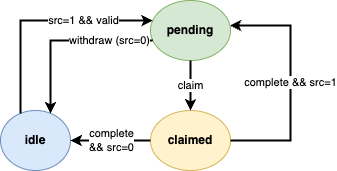
\includegraphics{plic-single-irq-fsm.png}
  \caption{PLIC 单中断源状态机}
  \label{fig:plic-single-irq-fsm}
\end{figure}

\section{Sv39 虚拟内存与内存管理单元}

本文实现了 RISC-V Sv39 虚拟内存方案~\cite{riscv2024priv}。Sv39 将 64 位虚拟地址的低 39 位划分为三级页号（VPN[2:0]，每级 9 位）与 12 位页内偏移，通过三级页表将虚拟页号翻译为 44 位物理页号（PPN）。当 satp 寄存器的 MODE 字段为 8 时启用 Sv39，satp.PPN 指向根页表的物理基地址。

内存管理单元由 TLB（Translation Lookaside Buffer）与 PTW（Page Table Walker）两个模块组成，IFU 与 LSU 各自实例化一套独立的 iTLB+PTW 和 dTLB+PTW，分别服务于取指地址翻译与访存地址翻译。两套 MMU 在结构上完全相同，仅在权限检查的具体位（IFU 检查 PTE.X，LSU 检查 PTE.R/PTE.W）上有所区别。

\subsection{TLB 设计}\label{sec:tlb}

TLB 采用 16 项全相联结构，以 VPN（27 位）作为 tag 进行匹配查询。查询时对所有表项并行比较，通过优先级编码器选中命中项，返回对应的 PPN 与页表标志位（flags）。sfence.vma 指令执行时，通过 flush 信号一次性失效全部表项。

TLB 的替换策略采用位矩阵 LRU（Bit-Matrix LRU）算法~\cite{belady1966replacement}。该算法使用一个 N×N 的位矩阵 M 记录表项间的访问先后关系：M[i][j] = 1 表示表项 i 比表项 j 更近被访问。当访问表项 k 时，将第 k 行全部置 1、第 k 列全部置 0，表示 k 成为最近访问项。需要淘汰时，选择行向量全为 0 的表项（即比所有其他表项都更早被访问的项）作为替换目标。算法伪代码如下：

\begin{lstlisting}[language=Python,caption={位矩阵 LRU 替换算法伪代码},label={lst:bit-matrix-lru}]
# 访问表项 k 时更新矩阵
def access(M, k, N):
    for j in range(N):
        M[k][j] = 1   # 第 k 行全部置 1
    for i in range(N):
        M[i][k] = 0   # 第 k 列全部置 0

# 选择 LRU 表项（行全零）
def find_lru(M, N):
    for i in range(N):
        if all(M[i][j] == 0 for j in range(N)):
            return i
\end{lstlisting}

位矩阵 LRU 的硬件实现仅需 N×(N-1)/2 个触发器（矩阵对角线恒为 0 且 M[i][j] = !M[j][i]，实际只需存储上三角），访问更新与 LRU 查询均可在单周期内完成，适合全相联结构的小容量 TLB。

\subsection{PTW 设计}\label{sec:ptw}

PTW 负责在 TLB 缺失时遍历内存中的三级页表。PTW 模块本身只关心一次完整的三级页表遍历算法；其对外请求/响应接口由前端 \lstinline|F1Stage| 外层的四态握手子 FSM 驱动，后者负责 TLB 缺失的启动、在途请求的 squash 协同与 iTLB 回填（详见~\ref{sec:ifu-mmu} 节）。PTW 采用九状态有限状态机实现：

\begin{figure}[H]
  \centering
  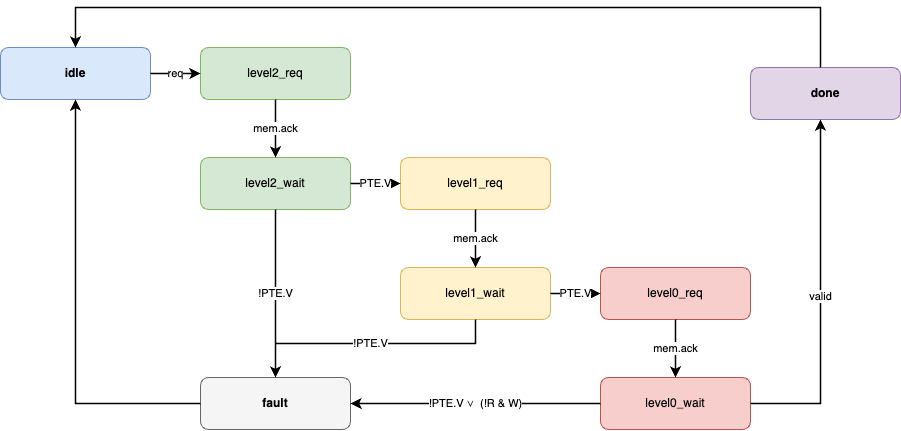
\includegraphics{ptw-fsm.png}
  \caption{PTW 页表遍历状态机}
  \label{fig:ptw-fsm}
\end{figure}

如图~\ref{fig:ptw-fsm} 所示，PTW 从 idle 状态接受请求后，依次访问第 2 级、第 1 级与第 0 级页表项。每一级的访问地址由上一级 PTE 中的 PPN 拼接当前级的 VPN 索引与 3 位字节偏移构成（每个 PTE 为 8 字节）。每级读取 PTE 后检查有效位（PTE.V）：若无效则进入 fault 状态报告页错误；若有效则继续下一级。第 0 级还额外检查权限合法性（不允许 !R \&\& W 的非法编码）。遍历成功后进入 done 状态，输出叶子 PTE 的 PPN 与 flags 供 TLB refill 使用。

\subsection{LSU 中的地址翻译}

LSU 的访存状态机采用与 IFU 相同（详见~\ref{sec:ifu-mmu} 节）的 TLB 优先策略：

如图~\ref{fig:lsu-fsm} 所示，ROB 发起访存请求后，LSU 首先判断 Sv39 是否启用。若未启用则直接使用虚拟地址进入 lsu\_req 访问 DCache 或外设端口；若启用则进入 tlb\_check 查询 dTLB。dTLB 命中时检查权限：Load 指令检查 PTE.R，Store 指令检查 PTE.W，权限不合法则报告 load page fault（mcause = 13）或 store page fault（mcause = 15）并回到 idle。权限合法则将翻译后的物理地址锁存，进入 lsu\_req。dTLB 缺失时启动 PTW，PTW 完成后 refill dTLB 并回到 tlb\_check 重新查询。

\begin{figure}[H]
  \centering
  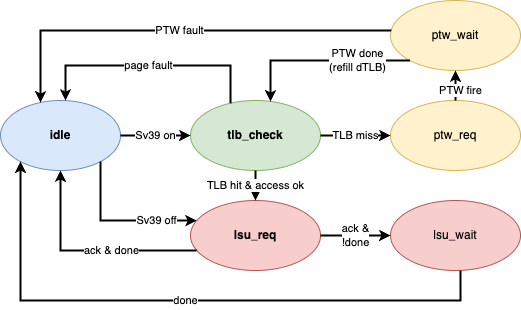
\includegraphics{lsu-fsm.png}
  \caption{LSU 访存状态机（含地址翻译）}
  \label{fig:lsu-fsm}
\end{figure}

lsu\_req 状态根据地址映射判断访问目标：若地址属于内存映射 I/O（MMIO, Memory-Mapped I/O）区域则通过外设端口（perip）访问，否则通过 DCache 端口访问。两条路径共享相同的握手逻辑：单周期完成时直接返回 idle，否则进入 lsu\_wait 等待数据就绪。Load 指令的返回数据根据访问宽度（byte/half/word/double）与符号扩展标志进行对齐提取与扩展后写回 PRF。

\section{本章小结}

本章介绍了 RISC-V M/S/U 三级特权架构、CSR 寄存器文件、精确异常、中断机制与 Sv39 虚拟内存的设计与实现。精确异常通过 ROB 顺序提交保证，异常仅在提交点生效；中断通过 CSRU 的挂起检测与 CommitStage 的注入机制实现，支持外部中断（PLIC）、定时器中断（CLINT/stimecmp）与软件中断三类来源，并通过 medeleg/mideleg 实现异常与中断的 M/S 两级委托。Sv39 虚拟内存由 TLB 与 PTW 两个模块实现，IFU 与 LSU 各自拥有独立的 iTLB/dTLB 与 PTW，采用“乐观路径先查 TLB、悲观路径回退到 PTW”的设计，在 TLB 命中时无额外延迟。

% !Mode:: "TeX:UTF-8"

\chapter{缓存设计}

\section{类 SRAM 总线协议}

处理器核心（IFU、LSU）与缓存之间的交互采用自定义的类 SRAM（SRAM-like）总线协议，而非直接使用 AXI4~\cite{arm2020axi4} 等复杂片上总线。这一设计的出发点是降低处理器核心侧的接口复杂度：AXI4 协议包含 5 个独立通道（AR、AW、W、R、B）与多种突发传输模式，对于处理器核心每次仅发起单拍读写的场景过于冗余；而类 SRAM 协议将读写统一到一组信号上，核心侧仅需驱动一个请求端口即可完成访存操作。

\begin{lstlisting}[language=Scala,caption={类 SRAM 总线接口定义},label={lst:sram-bundle}]
class SRAMBundle extends Bundle {
  val req   = Output(Bool())     // 请求有效
  val wen   = Output(Bool())     // 写使能（0=读，1=写）
  val size  = Output(UInt(...))  // 访问宽度
  val addr  = Output(UInt(...))  // 地址
  val wstrb = Output(UInt(...))  // 写字节掩码
  val wdata = Output(UInt(...))  // 写数据
  val ack   = Input(Bool())      // 请求被接受
  val done  = Input(Bool())      // 数据就绪 / 写完成
  val rdata = Input(UInt(...))   // 读数据
}
\end{lstlisting}

协议采用 req $\to$ ack $\to$ done 三阶段握手。图~\ref{fig:sram-read} 与图~\ref{fig:sram-write} 分别展示了一次读事务与一次写事务的时序波形。

\begin{figure}[H]
  \centering
  \begin{tikztimingtable}[xscale=1.2]
    clk   & 9{C} \\
    req   & L H H L L L L L L \\
    wen   & U L L U U U U U U \\
    size  & U D{2'b01} D{2'b01} U U U U U U \\
    addr  & U D{addr(A)} D{addr(A)} U U U U U U \\
    ack   & L L H L L L L L L \\
    done  & L L L L L H L L L \\
    rdata & U U U U U D{data(A)} U U U \\
  \end{tikztimingtable}
  \caption{类 SRAM 总线上的一次读事务}
  \label{fig:sram-read}
\end{figure}

\begin{figure}[H]
  \centering
  \begin{tikztimingtable}[xscale=1.2]
    clk   & 9{C} \\
    req   & L H H L L L L L L \\
    wen   & U H H U U U U U U \\
    size  & U D{2'b00} D{2'b00} U U U U U U \\
    addr  & U D{addr(B)} D{addr(B)} U U U U U U \\
    wdata & U D{data(B)} D{data(B)} U U U U U U \\
    ack   & L L H L L L L L L \\
    done  & L L L L L H L L L \\
  \end{tikztimingtable}
  \caption{类 SRAM 总线上的一次写事务}
  \label{fig:sram-write}
\end{figure}

如图~\ref{fig:sram-read} 所示，主设备发起读请求时拉高 req 并驱动 addr、wen=0、size 等信号，req 持续保持高电平直到从设备拉高 ack，此时两者同时拉低，完成一次请求握手（req-ack）。随后从设备在数据就绪时拉高 done 并在 rdata 上输出有效数据，完成数据响应。写事务（图~\ref{fig:sram-write}）的握手流程与读事务相同，区别在于 wen=1 且主设备额外驱动 wdata 与 wstrb。

该协议的核心设计在于将 req-ack 请求握手与 done 数据响应分离为两个独立阶段。这一分离带来两方面优势：

\begin{enumerate}
  \item 避免复杂协议。处理器核心与 L1 Cache 之间无需使用 AXI4 的五通道握手协议，仅需驱动 req 和检测 ack/done 两对信号，显著降低了核心侧的接口复杂度与控制逻辑面积。
  \item 保持流水能力。对于读操作，地址阶段（req-ack）与数据阶段（done）天然分离：ack 返回后地址已被缓存锁存，核心状态机可提前进入等待数据状态。当缓存命中时，ack 与 done 可在同一周期返回，实现单周期完成；当缓存缺失时，ack 先返回表示请求已接受，done 在缓存行填充完成后延迟返回。核心侧状态机无需区分命中与缺失，统一以“等待 done”收束。
\end{enumerate}

\subsection{Diplomacy 参数协商}

为使类 SRAM 总线能够融入 Rocket Chip~\cite{asanovic2016rocket} 的 Diplomacy 参数协商框架，本文为其实现了完整节点体系。接入 Diplomacy 后，Chisel elaboration 可理解为三个阶段：

\begin{enumerate}
  \item 将参数化硬件组织为有向无环图（DAG）；图中可存在多个参数源点，例如闭源 IP 核的接口参数通常不可被外部反向调整，只能作为约束源头。
  \item 框架沿连接关系遍历 DAG，完成参数协商并确定各模块实例的最终参数。
  \item 基于协商结果实例化具体硬件与 Bundle。其核心收益在于将“参数决定”前置为图级计算，避免在模块内部硬编码位宽与地址映射。
\end{enumerate}

在工程实现上，要接入 Diplomacy 必须补齐相应接口与节点抽象。本文具体实现包括：\lstinline|SRAMMasterPortParameters| 与 \lstinline|SRAMSlavePortParameters| 描述主从端口约束（地址范围、数据位宽等）；\lstinline|SRAMEdgeParameters| 在连线建立时由框架生成，封装协商后的 \lstinline|SRAMBundleParameters|；\lstinline|SRAMImp| 实现 \lstinline|SimpleNodeImp|，定义参数传递规则与硬件 Bundle 生成逻辑。在此基础上进一步派生 \lstinline|SRAMMasterNode|、\lstinline|SRAMSlaveNode|、\lstinline|SRAMNexusNode| 与 \lstinline|SRAMIdentityNode|，分别覆盖源节点、汇节点、多端口汇聚与透传场景。由于 Diplomacy 公开示例相对有限，本文实现过程主要参考《香山源码剖析》\cite{MaoDeCaoRISCVCPUXinPianSheJi} 中的方法，并在本项目中验证其可行性。

\subsection{SRAMToAXI4 桥接与缓存的双面接口}

类 SRAM 协议服务于处理器核心侧，而 SoC 互连采用 AXI4 协议，因此需要在两者之间进行协议转换。本文实现了通用的 \lstinline|SRAMToAXI4| 桥接模块，用于不经过缓存的直通路径（如外设端口）。桥接模块内部采用五状态 FSM（idle $\to$ readAddr $\to$ readData / write $\to$ writeResp），将 SRAM 的单拍读写映射为 AXI4 的单拍突发传输（len=0）。该模块基于 Diplomacy 的 \lstinline|MixedAdapterNode| 实现，上游为 SRAM 节点、下游为 AXI4 节点，参数在连接时自动转换。

ICache 与 DCache 本身也充当协议桥接的角色：面向处理器核心暴露类 SRAM 接口，接收单拍读写请求；面向 SoC 互连则通过 AXI4 接口与下级存储交互。缓存缺失时，缓存控制器通过 AXI4 Burst 传输（len > 0）从主存读取整条缓存行完成 refill；写回脏行时同样通过 AXI4 Burst 将整条缓存行写回主存。这一设计使处理器核心始终面对简洁的类 SRAM 接口，缓存内部负责单拍请求与突发传输之间的转换。

\section{PLRU 替换策略}

ICache 与 DCache 均为 4 路组相联结构（64 组，每组 4 路，缓存行 64 字节）。替换策略采用伪 LRU（Pseudo-LRU, PLRU）算法~\cite{belady1966replacement}，以较低的硬件开销近似 LRU 行为。

PLRU 使用一棵 $n-1$ 个节点的二叉树（4 路对应 3 个节点）记录访问方向。每个节点存储 1 位标志，指向“最近较少使用”的子树方向。如图~\ref{fig:plru} 所示，树的叶子节点对应 4 条缓存路，内部节点的标志位在每次访问时更新为指向另一侧，使得沿标志位路径走到的叶子即为待替换的路。

\begin{figure}[H]
  \centering
  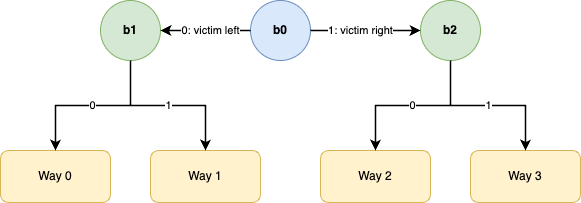
\includegraphics{plru.png}
  \caption{4 路 Pseudo-LRU 二叉树结构示意}
  \label{fig:plru}
\end{figure}

\begin{lstlisting}[language=Python,caption={PLRU 访问更新},label={lst:plru-access}]
def plru_access(tree: list[int], way: int):
    """访问 way 后更新 PLRU 树节点，使其指向远离被访问路的方向"""
    tree[0] = 1 if way in (0, 1) else 0  # 根节点
    tree[1 + way // 2] = 1 if way in (0, 2) else 0  # 子节点
\end{lstlisting}

\begin{lstlisting}[language=Python,caption={PLRU 替换选择},label={lst:plru-victim}]
def plru_victim(tree: list[int]) -> int:
    """沿树节点标志位从根到叶，返回待替换的路号"""
    if tree[0] == 0:  # go left
        return 0 if tree[1] == 0 else 1
    else:             # go right
        return 2 if tree[2] == 0 else 3
\end{lstlisting}

如代码~\ref{lst:plru-access} 所示，每次缓存命中时根据命中的路号更新树节点标志，使其指向远离被访问路的方向。如代码~\ref{lst:plru-victim} 所示，需要替换时沿树节点标志位从根到叶遍历，得到的叶子即为牺牲路。该算法仅需 3 位状态与简单的组合逻辑即可实现 4 路近似 LRU 替换，硬件开销远低于完整 LRU 所需的访问序记录。

\section{ICache}\label{sec:icache-fsm}

ICache 采用 VIPT（Virtually Indexed, Physically Tagged）结构，64 组 x 4 路 x 64 字节缓存行，总容量 16 KB。面向处理器核心提供类 SRAM 只读接口，面向 SoC 互连通过 AXI4 接口进行 refill。ICache 为只读缓存，不涉及写操作与脏行管理。

\begin{figure}[H]
  \centering
  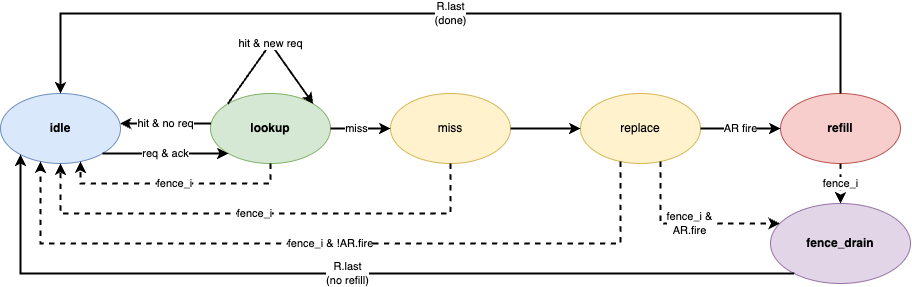
\includegraphics{icache-fsm.png}
  \caption{ICache 主状态机（虚线为 fence.i 相关跃迁）}
  \label{fig:icache-fsm}
\end{figure}

如图~\ref{fig:icache-fsm} 所示，ICache 的主状态机在原先五个状态的基础上，为支持前端对 \lstinline|fence.i| 的支持额外引入了 \lstinline|fence_drain| 状态，共六个状态：

\begin{enumerate}
  \item idle：等待请求。收到 req 时锁存地址（拆分为 tag、index、beat 偏移），返回 ack 并进入 lookup。
  \item lookup：用锁存的 tag 与 index 查询 tag RAM，4 路并行比较。若命中，直接从 cacheline 读出目标指令，返回 done 与 rdata。命中时若有新请求可直接锁存并停留在 lookup（lookup -> lookup 快速路径），实现连续命中的单周期吞吐。若缺失，记录 PLRU 选出的替换路号，进入 miss。
  \item miss -> replace：miss 为单周期过渡状态。replace 状态向 AXI4 AR 通道发起突发读请求（8 拍 x 8 字节 = 64 字节），AR 握手成功后进入 refill。
  \item refill：逐拍接收 AXI4 R 通道返回的数据并写入对应 cahcline。收到 R.last 后更新 tag RAM（写入新 tag、置 valid）、推进 PLRU 替换指针，返回 done 与 rdata，回到 idle。
  \item fence\_drain：专用于“AXI burst 已启动、但 fence.i 已到达”的中间状态。进入该状态后 ICache 消费完来自总线的突发读事务，但不再将数据回写到 tag RAM / cacheline，也不推进 PLRU，直到 \lstinline|r.last| 抵达后回到 idle。
\end{enumerate}

围绕 \lstinline|fence.i| 的处理贯穿了所有与总线相关的状态。当 \lstinline|fence_i| 脉冲到达时，ICache 会在同一拍把 \lstinline|tag_ram(*).valids| 全部清零——这使整个缓存在“语义”上立即变空。剩下的问题是如何与“已启动、无法撤销”的 AXI 事务共存：

\begin{enumerate}
  \item 在 idle / lookup / miss 三个状态下，ICache 尚未在 AXI 上发起任何 AR 握手，因此 \lstinline|fence_i| 到来时直接回到 idle；已失效的 tag RAM 保证下一次查询必然 miss 并重新从总线取指。
  \item 在 replace 状态下，AR 通道的 \lstinline|valid| 已经高起但是否握手取决于下游 \lstinline|ready|。若 \lstinline|fence_i| 与 \lstinline|ar.fire| 恰好同拍，则本次 burst 已经不可撤销，必须跳入 \lstinline|fence_drain| 把后续 R 拍全部吞掉；否则只需下一拍直接回 idle，AR 随之解挂。
  \item 在 refill 状态下，AR 必然已经 fire、R 通道正在返回，此时 \lstinline|fence_i| 强制进入 \lstinline|fence_drain|。此外还存在一种极端时序：若 \lstinline|fence_i| 与 \lstinline|r.last| 同拍到达，常规 refill 路径会在本拍把该行写入 tag RAM 并置 valid。为此，本设计采用优先级多路选择：“\lstinline|fence_i| clear valids” > “\lstinline|r.last| set valid”。
\end{enumerate}

这样，无论 \lstinline|fence.i| 在哪一个周期抵达，ICache 都能在至多一次额外 burst 的代价内回到“完全空缓存 + AXI 无事务”的干净状态，且整个过程不需要前端参与握手。前端因此可以对 \lstinline|fence.i| 完全保持透明：它像普通指令一样被取到 F3、送入后端，由后端 CommitStage 在提交时统一发出 \lstinline|fence_i| 脉冲与 \lstinline|io.flush|，其中 \lstinline|io.flush| 负责同周期清空整条取指流水。

\section{DCache}

DCache 同样采用 VIPT 结构，64 组 x 4 路 x 64 字节缓存行，总容量 16 KB。与 ICache 的关键区别在于 DCache 需要处理写操作，采用写回（write-back）策略，并引入 Write Buffer 与脏行写回机制。

\begin{figure}[H]
  \centering
  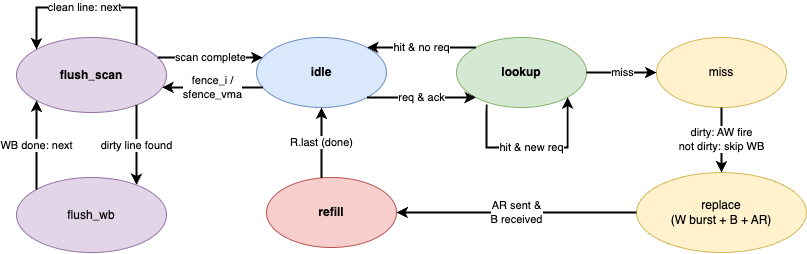
\includegraphics{dcache-fsm.png}
  \caption{DCache 主状态机}
  \label{fig:dcache-fsm}
\end{figure}

如图~\ref{fig:dcache-fsm} 所示，DCache 的主状态机包含七个状态：

\begin{enumerate}
  \item idle：等待请求。收到 \lstinline|fence.i| 时进入 flush 流程；正常请求时锁存地址与写控制信号（wen、wdata、wstrb），进入 lookup。\lstinline|sfence.vma| 仅作用于地址翻译缓存（TLB），不直接触发 DCache 刷写。
  \item lookup：4 路并行比较。命中时：若为读操作直接返回数据；若为写操作触发 Write Buffer——将写入目标（index、way、beat、wstrb、wdata）送入单项 Write Buffer，在下一周期由 Write Buffer 完成按字节掩码合并写入 data bank 并置脏位。Write Buffer 的引入使写命中不阻塞主 FSM，lookup 可立即接受下一请求。Write Buffer 还负责检测读写冲突：若新读请求与正在执行的 Write Buffer 写入地址重叠，则暂停接受请求直到 Write Buffer 完成。
  \item miss：PLRU 选出替换路后，检查 victimed 的 cacheline 是否为脏行。若脏则先通过 AXI4 AW 通道发起写回地址；若干净则跳过写回阶段。
  \item replace：该状态并行处理三个子阶段——（1）通过 AXI4 W 通道逐拍写回脏行数据；（2）等待 AXI4 B 通道确认写回完成；（3）通过 AXI4 AR 通道发起 refill 读请求。当 AR 发送完毕且 B 确认收到后进入 refill。
  \item refill：逐拍接收 R 通道数据写入 data bank。若原始请求为写操作，在目标 beat 位置将 refill 数据与写数据按字节掩码合并后写入。R.last 后更新 tag RAM（新 tag、valid、dirty 标志）、推进 PLRU 指针，返回 done 回到 idle。
  \item flush\_scan -> flush\_wb：由 \lstinline|fence.i|（或缓存维护触发）进入全缓存刷写流程。flush\_scan 逐组逐路扫描，遇到脏行则进入 flush\_wb 通过 AXI4 写回该行，写回完成后清除脏位并继续扫描，直到所有组路遍历完毕回到 idle。
\end{enumerate}

\section{指令-数据缓存一致性与 fence.i}

在冯·诺依曼架构~\cite{vonneumann1945edvac} 中，指令与数据共享同一地址空间；然而本处理器采用分离式 L1 缓存（ICache 与 DCache），二者之间不存在硬件一致性协议。这意味着当程序在运行时修改自身代码——即“自修改代码”（Self-Modifying Code）场景——时，ICache 与 DCache 之间会出现一致性问题。

一个典型的实例是 Bootloader 的快速启动路径：系统上电后，处理器从 XIP（Execute-In-Place）模式的 Flash 开始执行，Bootloader 将 Flash 中的应用程序映像搬运到 SDRAM 以获得更高的访问速度，随后跳转至 SDRAM 入口地址继续执行。其核心指令序列如下：

\begin{table}[H]
  \centering
  \caption{Bootloader 快速启动路径中的指令序列}
  \label{tbl:bootloader-seq}
  \begin{tabular}{cll}
    \toprule
    步骤 & 指令 & 含义 \\
    \midrule
    1 & \lstinline|sw inst, 0(sdram_addr)| & 将指令写入 SDRAM（经 DCache） \\
    2 & \lstinline|j sdram_addr| & 跳转至 SDRAM 入口执行 \\
    \bottomrule
  \end{tabular}
\end{table}

问题在于：步骤 1 的 \lstinline|sw| 指令将数据写入 DCache（写回策略下，脏行尚未写回 SDRAM）；步骤 2 的跳转触发 IFU 从 \lstinline|sdram_addr| 取指，而 IFU 只能访问 ICache 与下级存储，无法看到 DCache 中的脏数据。此时 ICache 未命中，从 SDRAM 读取到的仍是旧数据（全零或无效内容），导致处理器执行错误指令。

RISC-V 指令集架构通过 \lstinline|fence.i| 指令显式解决这一问题。正确的指令序列应为：

\begin{table}[H]
  \centering
  \caption{加入 fence.i 后的正确指令序列}
  \label{tbl:bootloader-fence}
  \begin{tabular}{cll}
    \toprule
    步骤 & 操作 & 含义 \\
    \midrule
    1 & \lstinline|sw inst, 0(sdram_addr)| & 将指令写入 SDRAM（经 DCache） \\
    2 & \lstinline|fence.i| & 同步指令流与数据流 \\
    3 & \lstinline|j sdram_addr| & 跳转至 SDRAM 入口执行 \\
    \bottomrule
  \end{tabular}
\end{table}

在本处理器的实现中，\lstinline|fence.i| 的执行分为两个阶段：

\begin{enumerate}
  \item DCache 刷写：DCache 进入 flush 流程（参见图~\ref{fig:dcache-fsm} 中 flush\_scan $\to$ flush\_wb 路径），逐组逐路扫描所有缓存行，将脏行通过 AXI4 写通道写回下级存储，确保所有已修改数据对外可见。
  \item ICache 失效：DCache 刷写完成后，ICache 将全部缓存行的 valid 位清零，迫使后续取指请求从下级存储重新加载。
\end{enumerate}

经过 \lstinline|fence.i| 的两阶段处理，步骤 1 写入 DCache 的指令数据已安全落入 SDRAM，而 ICache 的全部内容已失效。当步骤 3 跳转到 \lstinline|sdram_addr| 时，ICache 必然未命中，从 SDRAM 重新加载到正确的指令内容，程序得以正确执行。

需要指出的是，\lstinline|fence.i| 是一条代价较高的指令：它要求刷写整个 DCache 并失效整个 ICache，开销与缓存容量成正比。RISC-V 规范将其定义为“Zifencei”扩展而非基础指令集的一部分，正是考虑到在多核系统中维护指令-数据一致性有更高效的硬件机制（如 RISC-V CMO 扩展~\cite{riscv2023cmo}）。在本处理器的单核场景下，\lstinline|fence.i| 足以保证正确性，且实现简洁。

\section{DMA 与 DCache 的一致性}

上一节讨论的“指令-数据一致性”限定在单个 CPU 内部 ICache 与 DCache 之间；当处理器外部存在第二个主设备时，一致性问题会从“同一 core 内两份缓存”扩展到“核心侧 DCache 与外部主设备所见的主存”之间。本文在移植 xv6 时接入了 virtio-disk 控制器，其数据块传输由 DMA 引擎自行完成：DMA 引擎与 CPU 一同挂载到 AXI4 Crossbar 上（见图~\ref{fig:soc-arch}），以周期窃取（cycle stealing）的方式共用通往 SDRAM 的访存通道——CPU 未占用总线的拍次由 DMA 填入，二者对 Crossbar 而言是对称的主设备。

这一架构下 DMA 与 DCache 构成了两个能并发改写主存但彼此没有硬件协议同步的观察点，一致性缺口主要体现在两个对称方向：

\begin{enumerate}
  \item CPU $\to$ DMA 方向：xv6 在发起磁盘写请求前，先将待写入的数据填入驱动描述符指向的数据缓冲区；这条 \lstinline|sw| 经 DCache 采用的写回策略被吸收为脏行，尚未通过 AXI4 写通道落回 SDRAM。此时若 CPU 继续向 virtio 的 MMIO 通知寄存器写入 ``queue notify''，DMA 便会立即从 SDRAM 读取数据——读到的却是 DCache 背后的旧值，磁盘最终落盘的是错误内容。
  \item DMA $\to$ CPU 方向：磁盘读完成后 DMA 将数据直接写入 SDRAM 的目标缓冲区，并通过中断或 virtio 的 used ring 通知 CPU。若 CPU 在此前曾访问过同一地址范围，DCache 中已缓存了旧数据，后续的 \lstinline|lw| 将命中 DCache 而根本看不到 DMA 刚刚写入的新数据，内核读到的依然是未更新前的内容。
\end{enumerate}

两条路径共同揭示的问题是：DMA 事务的可见边界是 SDRAM，而 CPU 侧的观察窗口是 DCache；只要中间的写回/失效步骤未被显式触发，两方观察到的主存快照就会错位。

由于 xv6 的 virtio 驱动是本文自行移植并适配的，本文从软件侧对这一问题做了显式规避：在所有会触发或终结 DMA 事务的 MMIO 访问前后各插入一条 fence 指令。前端一侧的 fence 借助 DCache 主状态机的 \lstinline|flush_scan -> flush_wb| 路径（见图~\ref{fig:dcache-fsm}）将当前所有脏行写回 SDRAM，确保 CPU 已写入的数据对 DMA 可见；后端一侧的 fence 则同时起到作废 DCache 全部行的作用，迫使后续 \lstinline|lw| 重新从 SDRAM 读取 DMA 刚刚刷入的内容，从而覆盖 DMA $\to$ CPU 方向的可见性缺口。因 fence 的粒度是整个 DCache，配合 xv6 中 MMIO 访问频次不高的事实，这一软件方案在正确性上足以支撑 xv6 启动并稳定运行用户态程序，同时避免了在硬件上引入任何跨主设备的同步结构，复杂度代价最低。

这套以全局 fence 换取正确性的策略并非没有代价：每次磁盘块传输都触发一次整 cache 刷写，DCache 的时间局部性完全失效，对磁盘访问密集型负载（如文件系统压测、Shell 启动）的性能表现会显著恶化。更理想的做法是在硬件侧引入跨主设备的缓存一致性协议，例如类似 MESI~\cite{papamarcos1984mesi} 的嗅探（snoop）机制：DMA 发起访存时，Crossbar 以 bus snooping 将事务广播至 DCache，由 DCache 根据本地 tag 与行状态决定是转发脏数据、降级本地状态还是直接放行；CPU 写命中共享行时主动发出 invalidate 广播，使外部主设备感知。这样软件就无需在每次 MMIO 前后粘贴 fence，一致性由硬件按行粒度自动维护，对缓存局部性的损伤也被限制在真正发生冲突的单个缓存行上。这一方向涉及 AXI4-ACE~\cite{arm2023ace} / CHI~\cite{arm2023chi} 等一致性互连协议与多主设备仲裁的重新设计，已超出本文单核教学目标的范围，留作未来工作。

\section{本章小结}

本章围绕缓存子系统展开，首先介绍了面向处理器核心的类 SRAM 总线协议，其 req-ack-done 三信号握手机制在保持接口简洁的同时支持读地址与读数据的流水分离；随后描述了基于 Diplomacy 框架的参数协商与 SRAMToAXI4 总线桥的设计，使 ICache 与 DCache 对内呈现 SRAM 接口、对外通过 AXI4 Burst 完成 refill 与 writeback。在替换策略方面，采用 Pseudo-LRU 算法以 3 位状态实现 4 路近似最近最少使用替换，兼顾硬件面积与替换效果。ICache 采用六状态有限状态机实现只读缓存逻辑，其中专用的 \lstinline|fence_drain| 状态将 \lstinline|fence.i| 与 inflight 的 AXI burst 的收敛完全封闭在缓存内部，使前端不再需要为 \lstinline|fence.i| 维护额外的握手或粘滞位；DCache 则通过七状态有限状态机支持写回策略、Write Buffer 优化及全缓存刷写。最后讨论了分离式 ICache 与 DCache 架构下的指令-数据一致性问题，说明了 \lstinline|fence.i| 指令通过 DCache 刷写加 ICache 失效两阶段操作保证自修改代码的正确执行；以及接入 virtio-disk 后 DMA 与 DCache 之间的可见性缺口，说明了本文以 MMIO 前后软件 fence 规避该问题的工程取舍，并指出引入类 MESI 的硬件一致性协议是更理想的长期方向。

% !Mode:: "TeX:UTF-8"

\chapter{仿真平台}

处理器设计的正确性高度依赖仿真验证。本章介绍基于 Verilator 与 C++20 构建的仿真平台，涵盖简易调试器、执行追踪、差分测试、快照回放及外设可视化等功能，为处理器开发全流程提供调试与验证支撑。

\section{仿真平台整体架构}

仿真平台以 C++20 编写，遵循 Google C++ Style Guide~\cite{google_cpp_styleguide} 编码规范，使用 CMake 构建系统管理依赖。整体架构如图~\ref{fig:sim-arch} 所示，由以下核心组件构成：

\begin{figure}[H]
  \centering
  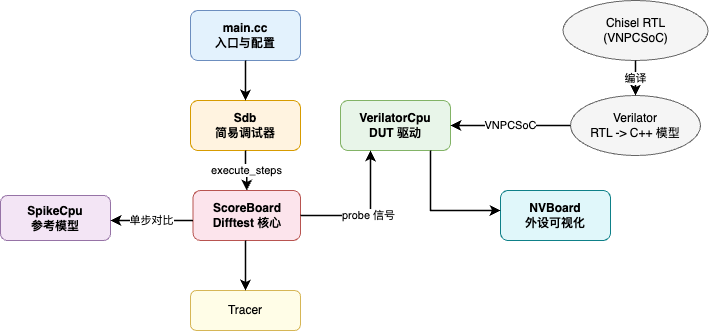
\includegraphics{sim-arch.png}
  \caption{仿真平台整体架构}
  \label{fig:sim-arch}
\end{figure}

Verilator 将 Chisel 生成的 Verilog 网表编译为 C++ 仿真模型 \lstinline|VNPCSoC|。\lstinline|VerilatorCpu| 封装该模型并驱动时钟信号，通过 Chisel 的 probe 机制从 RTL 中导出 PC、通用寄存器、CSR、提交有效信号等观测点，供上层调试与比对使用。\lstinline|ScoreBoard| 是差分测试与追踪记录的核心枢纽：每条指令提交后，它同步驱动参考模型 \lstinline|SpikeCpu| 执行同一条指令，比较两侧架构状态，并将执行信息写入各类 Tracer 的环形缓冲区。\lstinline|Sdb|（Simple Debugger）提供交互式调试界面，支持单步执行、断点、监视点与表达式求值。命令行标志 \lstinline|--batch| 可使仿真在无人值守模式下全速运行，\lstinline|--wave| 可按需开启波形记录。

\section{简易调试器}

Sdb 提供类 GDB 的交互式命令行界面，基于 GNU Readline 实现命令补全与历史记录。支持的调试命令包括：

\begin{table}[H]
  \centering
  \caption{Sdb 调试命令列表}
  \label{tbl:sdb-cmds}
  \begin{tabular}{ccl}
    \toprule
    命令 & 缩写 & 功能 \\
    \midrule
    \lstinline|continue| & \lstinline|c| & 继续执行直到断点或程序结束 \\
    \lstinline|step| & \lstinline|si| & 单步执行 N 条指令（默认 1） \\
    \lstinline|info r| & & 显示所有通用寄存器与 PC \\
    \lstinline|info w| & & 列出所有监视点 \\
    \lstinline|print| & \lstinline|p| & 对表达式求值并输出 \\
    \lstinline|examine| & \lstinline|x| & 查看指定地址处的内存内容 \\
    \lstinline|watch| & \lstinline|w| & 添加监视点，表达式值变化时暂停 \\
    \lstinline|break| & \lstinline|b| & 在指定地址设置断点 \\
    \lstinline|delete| & \lstinline|d| & 删除指定监视点 \\
    \bottomrule
  \end{tabular}
\end{table}

\subsection{表达式求值引擎}

Sdb 内置了一个完整的表达式求值引擎，使用 Flex~\cite{flex_manual} 进行词法分析、Bison~\cite{bison_manual} 进行语法分析。该引擎支持以下语法特性：

\begin{itemize}
  \item 字面量：十进制整数、十六进制整数（\lstinline|0x| 前缀）。
  \item 寄存器引用：\lstinline|$pc|、\lstinline|$ra|、\lstinline|$sp| 等，通过 \lstinline|AbstractCpu::value()| 接口读取当前 CPU 状态。
  \item 算术运算：\lstinline|+|、\lstinline|-|、\lstinline|*|、\lstinline|/|。
  \item 比较运算：\lstinline|==|、\lstinline|!=|、\lstinline|<|、\lstinline|<=|、\lstinline|>|、\lstinline|>=|。
  \item 逻辑运算：\lstinline!&&!、\lstinline!||!。
  \item 一元运算：负号 \lstinline|-|、解引用 \lstinline|*addr|（读取指定地址的内存值）。
\end{itemize}

表达式求值贯穿调试器的多个功能：\lstinline|print| 命令直接求值输出，\lstinline|examine| 命令使用表达式计算起始地址，\lstinline|watch| 命令在每步执行后重新求值以检测变化。

\section{执行追踪}

仿真平台实现了四类追踪器（Tracer），均基于泛型环形缓冲区 \lstinline|RingBuf<T>| 存储最近的追踪记录。环形缓冲区采用固定容量、覆写最旧记录的策略，在常数内存开销下保留最近的执行历史，供错误发生时回溯分析：

\begin{enumerate}
  \item ITrace(Instruction Tracer) 记录每条提交指令的 PC、机器码与反汇编文本。反汇编由 Spike 的内置反汇编器生成，保证与参考模型的指令解读一致。当 difftest 失败时，ITrace 的输出可直接定位出错指令及其上下文。
  \item MTrace(Memory Tracer) 记录所有非 MMIO 的 load/store 操作，包括 PC、访存方向（读/写）、物理地址、数据值与访问宽度。对于 load 指令，数据值取自 DUT 的内存模型；对于 store 指令，数据值取自参考模型的寄存器。MTrace 对缓存一致性问题与访存相关 bug 的定位尤为有效。
  \item DTrace(Device Tracer) 专门记录 MMIO 区域的访问，格式与 MTrace 相同但独立存储。MMIO 访问具有副作用（如串口发送、定时器读取），其正确性无法通过简单的内存比对验证，因此单独追踪便于开发者审查外设交互序列。
  \item FTrace(Function Tracer) 从 ELF 文件的符号表中加载函数名与地址映射，在运行时根据指令助记符识别函数调用（\lstinline|jal|/\lstinline|jalr| 且 \lstinline|rd=ra|）与返回（\lstinline|ret|），维护调用深度计数器，生成带缩进的调用链记录。FTrace 对操作系统启动流程的调试尤为有用：当程序陷入死循环或异常跳转时，调用链能清晰展示控制流的偏离点。
\end{enumerate}

\section{差分测试}\label{sec:difftest}

差分测试（Differential Testing，Difftest）\cite{you2025difftest} 是本仿真平台最核心的验证手段。

\subsection{理论基础：处理器的双层状态机模型}

从抽象层次看，处理器本质上是一个状态机，其状态可分为两个层次：

\begin{enumerate}
  \item ISA 状态（Instruction Set Architecture State）：程序员可见的架构状态，包括程序计数器 PC、32 个通用寄存器、CSR 寄存器以及内存内容。ISA 规范严格定义了每条指令对这些状态的转移规则，任何符合规范的实现——无论是单周期、多周期还是乱序流水线——在执行同一条指令后都必须产生相同的 ISA 状态。
  \item 物理状态（Physical/Microarchitectural State）：硬件实现的微架构状态，包括流水线寄存器、重排序缓冲区、缓存行、分支预测器历史等。这些状态对程序员不可见，不同微架构实现之间存在本质差异。
\end{enumerate}

程序员编写软件时只需关心 ISA 状态——这正是 ISA 作为硬件与软件之间契约的核心含义。即便存在诸如 \lstinline|fence.i| 这样涉及微架构行为的指令，其语义仍然是在 ISA 层面定义的（“使后续取指看到此前的数据写入”），而非暴露具体的缓存实现细节。

基于这一认识，差分测试的思路自然浮现：如果存在一个公认正确的 ISA 状态机作为参考，让待验证的处理器（DUT）与之逐条指令执行同一程序，每步比较 ISA 状态，若始终一致，即可断言 DUT 的实现在 ISA 语义上是正确的。RISC-V 基金会维护的官方指令集模拟器 Spike~\cite{spike2026} 正是这样一个标准的 ISA 参考状态机：它严格按照 RISC-V 规范实现每条指令的状态转移，不涉及任何微架构细节，是差分测试的理想参考模型。

\subsection{参考模型集成}

本平台以静态链接方式集成 Spike（\lstinline|spike::riscv| 库），而非通过动态库加载，使仿真平台的部署更为简洁。\lstinline|SpikeCpu| 类封装了 Spike 的 \lstinline|sim_t|、\lstinline|processor_t| 与 \lstinline|state_t|，并按照 SoC 的实际地址映射（Flash 位于 \lstinline|0x3000_0000|、SDRAM 位于 \lstinline|0x8000_0000| 等）初始化 Spike 的内存布局，确保两侧的初始 ISA 状态完全一致。

\subsection{比对流程}

差分测试的执行流程由 \lstinline|ScoreBoard::scoreboard()| 驱动，每条指令提交后执行以下步骤：

\begin{enumerate}
  \item DUT 侧：\lstinline|VerilatorCpu::step()| 驱动时钟直到 \lstinline|probe_valid| 信号有效，表示一条指令已提交。通过 probe 信号读取 DUT 的 PC、下一 PC（\lstinline|dnpc|）、机器码、通用寄存器与 CSR——这些正是 ISA 状态的完整快照。
  \item 参考模型侧：调用 \lstinline|SpikeCpu::step()| 执行同一条指令，Spike 按照 ISA 规范更新其内部状态。
  \item ISA 状态比对：\lstinline|check_regs()| 逐一比较 DUT 与 Spike 的下一 PC、32 个通用寄存器（\lstinline|x1|--\lstinline|x31|）以及关键 CSR（\lstinline|mtvec|、\lstinline|mepc|、\lstinline|mcause|、\lstinline|mtval|、\lstinline|mstatus| 等），任一不匹配即判定 DUT 的 ISA 行为偏离规范。
\end{enumerate}

\subsection{MMIO 特殊处理}

MMIO 访问具有副作用且地址空间在 DUT 与 Spike 之间不一定对等，因此需要特殊处理。当 DUT 的 \lstinline|is_mmio| 信号有效时，ScoreBoard 不调用 \lstinline|golden_.step()|，而是：

\begin{itemize}
  \item 对 MMIO load：从 DUT 的目的寄存器读取实际值，写入 Spike 对应寄存器，使两侧对齐。
  \item 对 MMIO store：记录到 DTrace，不修改 Spike 内存。
  \item 最后将 Spike 的 PC 强制设置为 DUT 的 \lstinline|dnpc|，跳过 Spike 对该指令的执行。
\end{itemize}

这种“DUT 主导、参考模型跟随”的策略确保了 MMIO 访问不会导致两侧状态分叉。

\subsection{失败诊断}

当 difftest 检测到不一致时，\lstinline|ScoreBoard::dump_traces()| 按序输出四类 Tracer 的环形缓冲区内容，并以表格形式并排展示 DUT 与 Spike 的寄存器与 CSR 状态，用 \lstinline|<--- MISMATCH| 标记不一致项。开发者可据此快速定位出错指令及其影响的架构状态。

\section{LightSSS 快照回放}

在长时间仿真过程中，某些 bug（如总线死锁、缓存状态机卡死）可能在数百万周期后才触发，此时重新从头仿真并开启波形记录的开销极为高昂。LightSSS（Lightweight Simulation Snapshot）利用操作系统的 \lstinline|fork()| 系统调用实现轻量级快照功能：

\begin{enumerate}
  \item 周期性快照：仿真每执行一定数量的指令后，调用 \lstinline|fork()| 创建子进程。由于 \lstinline|fork()| 采用写时复制（Copy-on-Write）语义，快照的创建几乎零开销——父子进程共享相同的物理内存页，仅在后续写入时才触发页复制。
  \item 异常检测：当仿真检测到异常状态（如 \lstinline|VerilatorCpu::step()| 超过最大周期数仍未收到 \lstinline|probe_valid|，表明总线可能死锁），触发快照回放机制。
  \item 死亡回放：系统回退到最近一个 checkpoint 对应的子进程，在该快照上重新执行，但此次开启波形记录（\lstinline|--wave|）与全部 Tracer，以最小的时间窗口捕获 bug 触发前后的完整信息。
\end{enumerate}

\begin{figure}[H]
  \centering
  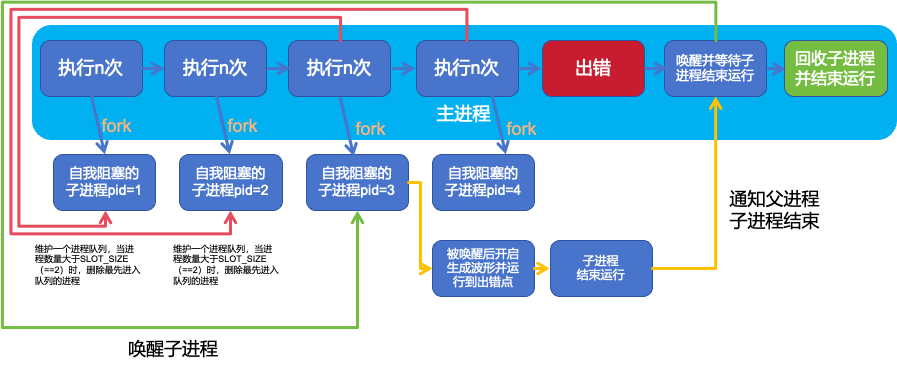
\includegraphics{lightsss.png}
  \caption{LightSSS 快照回放原理示意}
  \label{fig:lightsss}
\end{figure}

如图~\ref{fig:lightsss} 所示，主进程每执行 N 条指令后调用 \lstinline|fork()| 创建一个自我阻塞的子进程作为快照，并维护一个固定大小的进程队列，当快照数量超出上限时淘汰最早的快照。当主进程检测到仿真出错时，唤醒最近的快照子进程，该子进程开启波形记录并重新运行到出错点，完成“死亡回放”后通知父进程回收资源。这一机制的关键优势在于：正常仿真时无需开启波形记录（可提升 5--10 倍仿真速度），仅在 bug 触发时才回放并记录，大幅缩小了仿真日志与波形文件的体积。

\section{NVBoard 外设可视化}\label{sec:nvboard-vis}

仿真平台集成了 NVBoard(NJU Virtual Board) 虚拟开发板，通过将 RTL 顶层的 GPIO、七段数码管、PS2 键盘、VGA 显示与 UART 串口等外设信号绑定到 NVBoard 的虚拟引脚，在仿真过程中实时渲染外设状态。通过命令行标志 \lstinline|--nvboard| 启用。

对于 UART 输出，仿真平台实现了 \lstinline|UartTxDecoder| 模块，在仿真时钟域内按 8N1（8bit data, no parity, 1bit stop）格式解码串口帧。由于仿真平台采用单时钟域，“与裸机程序约定相同波特率”等价于“约定相同分频系数（\lstinline!div = (dlm << 8) | dll!）”。波特率与分频系数的换算公式如下：

\[
\mathrm{Divisor} = \frac{\mathrm{system\ clock\ frequency}}{16 \times \mathrm{desired\ baud\ rate}}
\]

软件侧 UART 初始化如代码~\ref{lst:uart-init} 所示。这里 soc 侧的分频系数 \lstinline|div = 1|，只需让 NVBoard 满足相同的采样频率即可正常收发字符。

\begin{lstlisting}[language=C,caption={UART 初始化与波特率分频配置示例},label={lst:uart-init}]
static void uart_init(void) {
  volatile char *lcr = (volatile char *)UART_LCR;
  volatile char *dll = (volatile char *)UART_DLL;
  volatile char *dlm = (volatile char *)UART_DLM;
  volatile char *fcr = (volatile char *)UART_FCR;
  *lcr = LCR_DLAB;
  *dll = 0x01; // Divisor Latch Low
  *dlm = 0x00; // Divisor Latch High
  *lcr = LCR_8N1; // 8N1, disable setting BAUD rate
  *fcr = FCR_FIFO_ENABLE | FCR_RX_RESET | FCR_TX_RESET;
}
\end{lstlisting}

图~\ref{fig:nvboard} 展示了 NVBoard 虚拟开发板的运行截图，整个程序运行在 RT-Thread~\cite{yi2023rtthread} 实时操作系统之上。左上角为 GPIO 区域，七段数码管显示学号后 8 位；右上角为 UART 串口终端与 PS/2 键盘回显，可见 RT-Thread 的 msh（Mini Shell）命令行界面及其内置命令列表；左下角为 VGA 显示区域，正在运行贪吃蛇程序；右下角为 PS/2 虚拟键盘，用于向处理器发送按键扫描码。各外设在仿真过程中实时更新，为软硬件协同调试提供直观的可视化反馈。

\begin{figure}[H]
  \centering
  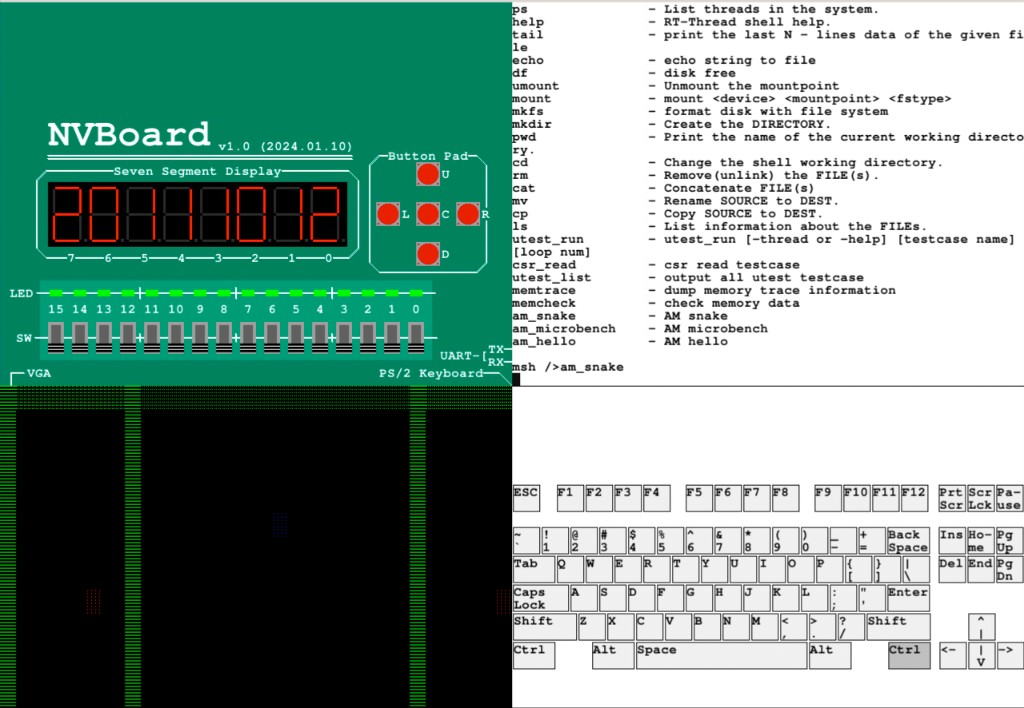
\includegraphics[width=0.85\textwidth]{nvboard.jpg}
  \caption{NVBoard 虚拟开发板运行 RT-Thread 操作系统上的贪吃蛇程序}
  \label{fig:nvboard}
\end{figure}

\section{本章小结}

本章介绍了基于 Verilator 与 C++20 构建的仿真验证平台。该平台以 Google C++ Style Guide 为编码规范，围绕“调试—追踪—比对—回放—可视化”五个维度构建了完整的验证工具链：Sdb 简易调试器提供交互式单步执行与断点调试，内置基于 Flex/Bison 的表达式求值引擎；四类 Tracer（ITrace、MTrace、DTrace、FTrace）基于环形缓冲区记录指令、访存、MMIO 与函数调用历史；差分测试以 Spike 为参考模型，逐条指令比对架构状态，MMIO 访问采用 DUT 主导策略保持两侧同步；LightSSS 利用 \lstinline|fork()| 写时复制实现轻量级快照，在 bug 触发时自动回放并开启波形记录；NVBoard 集成提供 GPIO、UART、VGA 等外设的实时可视化。上述工具的协同使用，使得从功能验证到性能调优的全流程均有据可查、有迹可循。

% !Mode:: "TeX:UTF-8"

\chapter{性能评估}

为定量评估本处理器在典型工作负载下的微架构行为，本章在 RTL 仿真环境中选取三组广泛使用的基准程序进行端到端性能测试，覆盖综合性整数基准（MicroBench）、经典系统编程基准（Dhrystone~\cite{weicker1984dhrystone}）与嵌入式行业标准基准（CoreMark~\cite{coremark2009}）。在此基础上，通过在 RTL 与仿真器两侧协同添加的性能计数器，从 IPC、分支预测命中率、缓存命中率与平均访存时间（AMAT, Average Memory Access Time）、前端取指率、指令混合等多个维度对处理器行为进行定量分析。

\section{实验方法与计数器实现}

\subsection{仿真环境}

性能评估在本文基于 Verilator 构建的 C++20 仿真平台上运行，所有被测程序均以 rv64im\_zicsr\_zifencei~\cite{riscv2024unpriv} 为目标架构交叉编译，运行于 Abstract Machine~\cite{nju_abstract_machine} 抽象层提供的裸机环境中，不经操作系统调度。裸机程序通过执行 \lstinline|ebreak| 实现停机。

\subsection{计数器架构}

性能计数器采用 DPI-C 事件方案实现。提交相关事件（commit、branch、branch\_mispredict、flush 以及按 \lstinline|InstType| 划分的十类指令混合）与缓存相关事件（访问、命中、未命中、Miss Cycles、IFU 输出有效、IFU 停顿等）均通过一个仅用于仿真的 SystemVerilog~\cite{ieee2017systemverilog} 外部模块 \lstinline|PerfEventHelper| 在触发时钟沿调用 DPI-C~\cite{ieee2017systemverilog} 函数 \lstinline|npc_perf_event(id)|，由 C++ 侧 \lstinline|PerfCounters| 统一累加。

这种“事件导出、仿真侧聚合”的方式与业界主流开源处理器性能监控单元（PMU, Performance Monitoring Unit~\cite{arm2024armArm}~\cite{wang2023xiangshan}）的观测思路一致：将观测逻辑尽量与处理器主数据通路解耦，降低统计机制对微架构实现的侵入性。后续可扩展为纯 RTL 实现的 PMU。

\subsection{指标定义}

本章使用的关键指标定义如下：

\begin{table}[H]
  \centering
  \caption{性能评估关键指标定义}
  \label{tbl:perf-metrics}
  \begin{tabular}{cl}
    \toprule
    指标 & 定义 \\
    \midrule
    IPC & 已提交指令数 / 复位释放后的总仿真周期数 \\
    Branch Hit Rate & 正确预测的控制流指令数 / 控制流指令总数 \\
    Cache Hit Rate & 缓存命中次数 / 缓存访问次数 \\
    AMAT & $1 + \text{缺失周期数}/\text{访问次数}$（命中按 1 周期计） \\
    IFU Stall Ratio & IFU 未输出有效指令的周期数 / 总周期数 \\
    \bottomrule
  \end{tabular}
\end{table}

其中 AMAT 的定义将命中基准归一化为 1 个周期，缺失时新增的等待周期全部计入访问摊销。由于本实现中缓存命中即可在同一周期返回数据，该公式等价于 $\text{命中延迟} \times \text{命中率} + \text{缺失延迟} \times \text{缺失率}$。

\subsection{基准程序简介}

为覆盖不同维度的处理器行为，本实验选取的三组基准程序在设计思路上互为补充，分别代表“算法异质性”、“系统编程典型语句”与“嵌入式工业标准”三类不同的评测视角：

\begin{itemize}
  \item MicroBench~\cite{microbench2024}：南京大学体系结构教学组设计的基准测试集，包含 10 个功能各异的子测试——\lstinline|qsort| 快速排序、\lstinline|queen| 位运算实现的 n 皇后、\lstinline|bf| Brainf**k 解释器、\lstinline|fib| 矩阵法 Fibonacci、\lstinline|sieve| Eratosthenes 筛法、\lstinline|15pz| A* 求解 4×4 数码问题、\lstinline|dinic| 二分图最大流、\lstinline|lzip| 压缩、\lstinline|ssort| 后缀排序与 \lstinline|md5| 哈希。这些子测试覆盖排序、回溯搜索、解释器、动态规划、图算法、压缩与密码学计算等差异显著的算法形态，可暴露处理器在不同控制流与访存模式下的稳态行为。MicroBench 提供 \lstinline|test|/\lstinline|train|/\lstinline|ref|/\lstinline|huge| 四档输入规模（动态指令数约 300K / 60M / 2B / 50B），选用 \lstinline|train| 档是因为运行时间适中且能合理展示本设计的性能。
  \item Dhrystone~\cite{weicker1984dhrystone}：由 Weicker 于 1984 年提出的综合整数基准，无浮点（本设计不支持浮点）、无 I/O、不依赖操作系统。主循环由若干典型系统编程语句构成，包括结构体字段读写、字符串库函数 \lstinline|strcmp|/\lstinline|strcpy|、过程调用与条件分支，旨在反映通用整数处理的指令混合与访存密度。本实验使用 Dhrystone v2.2。
  \item CoreMark~\cite{coremark2009}：EEMBC 于 2009 年发布的嵌入式行业标准基准，由链表插入/删除/查找、矩阵乘法/反转与状态机 CRC 三类核心算法组成。EEMBC 通过算法间的数据依赖与运行时种子参数显著抑制了编译器的常量折叠、死代码消除等优化空间，使评分难以通过单纯的编译技巧“作弊”，从而较 Dhrystone 更能反映核心微架构的真实性能。
\end{itemize}

所有被测基准程序均以 C 语言编写，使用 \lstinline|riscv64-none-elf-gcc| 15.2.0 交叉编译，编译参数统一为 \lstinline|-O2|。

\subsection{基准程序配置}

考虑到 RTL 仿真速度约为 0.1 MIPS 量级，若采用 benchmark 默认配置则单次运行可能需要数小时甚至数十小时，严重影响实验迭代效率。因此本实验对各基准程序的规模参数进行了合理压缩，具体配置如下：

\begin{table}[H]
  \centering
  \caption{基准程序规模与配置说明}
  \label{tbl:perf-bench-config}
  \begin{tabular}{cll}
    \toprule
    基准 & 规模 & 说明 \\
    \midrule
    MicroBench~\cite{microbench2024} & \lstinline|train| & Microbench 的 \lstinline|train| 动态指令数约为 60M，本实验实际跑出约 73M 提交指令 \\
    Dhrystone~\cite{weicker1984dhrystone} & 140000 iter & Dhrystone 140,000 iter 与 Microbench train 的动态指令数，数量级相同 \\
    CoreMark~\cite{coremark2009} & 200 iterations & CoreMark 200 iterations 与 Microbench train 的动态指令数，数量级相同 \\
    \bottomrule
  \end{tabular}
\end{table}

需要说明的是，基准程序规模的压缩仅影响数据工作集与运行时长，不改变其指令混合特征与访存模式，因此对 IPC、命中率、分支预测率等微架构指标的评估结论具有代表性。

\section{总体性能结果}\label{sec:perf-pipeline}

三组基准程序的整体执行统计如表~\ref{tbl:perf-overview} 所示。

\begin{table}[H]
  \centering
  \caption{基准程序整体执行统计}
  \label{tbl:perf-overview}
  \begin{tabular}{lrrrr}
    \toprule
    基准 & 周期数 & 提交指令数 & IPC & CPI \\
    \midrule
    MicroBench (train) & 155\,612\,739 & 73\,354\,577 & 0.4714 & 2.12 \\
    Dhrystone & 142\,530\,258 & 64\,453\,461 & 0.4522 & 2.21 \\
    CoreMark (200 iter) & 129\,901\,647 & 71\,795\,820 & 0.5527 & 1.81 \\
    \bottomrule
  \end{tabular}
\end{table}

三组负载的 IPC 分别为 0.47、0.45 与 0.55，CPI 对应为 2.12、2.21 与 1.81；IPC 随负载特性分层出现，其中 CoreMark 由于存在较多长直线段和极高的 ICache 命中率（见表~\ref{tbl:perf-icache}），可被流水前端连续供应指令，因而取得最高的 IPC。MicroBench train 与 Dhrystone 的 IPC 接近（0.4714 vs 0.4522），两者差距主要来自前端停顿比例与分支误预测惩罚的不同。

从前后端协同角度看，可以引入一个反映前后端协同效率的指标 \lstinline|commit / ifu_deliver|（\lstinline|ifu_deliver| 见表~\ref{tbl:perf-fe-events}）：其中 \lstinline|ifu_deliver| 是前端 IFU 在 F3 段成功交付给后端的指令数（即“塞入”指令队列的有效指令数），\lstinline|commit| 则是后端 ROB 最终顺序提交并写回架构状态的指令数。两者之差对应“被前端发出，但因分支误预测、异常或 \lstinline|fence.i| / CSR 写等 serializing 事件而中途被流水线 flush 掉的指令”，因此该比值在理想情况下应趋近于 1，比值越接近 1 说明前端推测发出的指令越少被作废，前后端的协同效率越高。

本实现下该比值在三组负载上分别为 MicroBench $\approx$ 0.877（73\,354\,577 / 83\,659\,693）、Dhrystone $\approx$ 0.911（64\,453\,461 / 70\,759\,218）与 CoreMark $\approx$ 0.908（71\,795\,820 / 79\,038\,883），整体稳定在 0.88--0.91 区间。换言之，每 100 条由前端送往后端的指令中约有 9--12 条最终被作废。结合本处理器的流水线深度可对这一损耗给出合理解释：前端 F1/F2/Fp/F3 共 4 级，后端经译码、重命名、分派、发射、执行、写回到提交共约 7 级，整条流水线深度达到 4+7 级；当后端在提交点确认一次分支误预测时，CommitStage 通过 \lstinline|io.flush| 在一个周期内同时清空前端 IFU 的所有流水段、指令队列以及后端从重命名到写回的所有流水段，单次 flush 损失的有效工作量近似等于流水线深度。该比值反映了“全流水线 flush”恢复策略放大了每次分支误预测的代价。

要进一步提升该比值，可考虑降低单次 flush 的惩罚：例如分支预测出错误，可以在执行阶段就对前端做重定向，而不是要等到提交时再对前端做重定向，降低分支指令带来的惩罚。

\section{前端事件分析}\label{sec:perf-fe-breakdown}

为进一步定位前端中各段的开销，表~\ref{tbl:perf-fe-events} 列出了前端 PerfEvent 在三组负载上的计数。事件含义与指标定义见表~\ref{tbl:perf-metrics}。需要说明的是，本实验运行于 Abstract Machine 裸机环境，未配置页表也未启用 Sv39 分页，iTLB 查表全程被旁路，因此 F1 TLB-miss 计数对所有负载均为 0，下表不再单独列出该列。

\begin{table}[H]
  \centering
  \caption{前端各段事件计数}
  \label{tbl:perf-fe-events}
  \begin{tabular}{lrrrr}
    \toprule
    基准 & IFU deliver Inst. & IFU stall Cyc. & F2 ICache wait Cyc. & Fp resp wait Cyc. \\
    \midrule
    MicroBench (train) & 83\,659\,693 & 49\,889\,859 & 20\,745\,873 & 6\,818 \\
    Dhrystone (140 000) & 70\,759\,218 & 58\,294\,840 & 15\,433\,031 & 1\,933 \\
    CoreMark (200 iter) & 79\,038\,883 & 44\,685\,323 & 4\,754\,811 & 4\,041 \\
    \bottomrule
  \end{tabular}
\end{table}

主要观察：

\begin{enumerate}
  \item ICache 是首要前端停顿源：\lstinline|F2 ICache wait| 在所有负载上都是前端停顿周期的主导项。其中 MicroBench train 的 ICache 等待周期达到 20.7M，占总周期的 13.3\%，对应 IFU 总停顿比 32.06\%（49.9M / 155.6M 周期）；Dhrystone 的 ICache 等待周期为 15.4M，占总周期的 10.8\%，对应 IFU 总停顿比 40.90\%（58.3M / 142.5M 周期）；CoreMark 由于工作集小、ICache 命中率几近 100\%，ICache 等待仅 4.75M 周期、占总周期 3.66\%，对应 IFU 总停顿比 34.40\%（44.7M / 129.9M 周期）。这说明 ICache 等待是前端停顿的主导但非全部，剩余部分由 Fp 段排队、后端反压与重定向气泡构成。这一观察表明前端剩余性能主要受制于缓存与主存之间的传输带宽，而非流水线结构本身。
  \item Fp 响应等待极少：\lstinline|Fp resp wait| 在所有负载上均不到 7\,000 周期（最高为 MicroBench 的 6\,818），表明在典型负载下 ICache 的访问延迟大多可以被流水覆盖，Fp 作为“in-flight 缓冲段”承担了绝大多数 cache 响应周期的吸收工作。
\end{enumerate}

\section{分支预测性能分析}

表~\ref{tbl:perf-bp} 展示了 GShare + IJTC + RAS 组合预测器在三组负载中的表现。RAS 的 push/pop 挂在 \lstinline|io.out.fire| 而非 F3 出现的时刻，这使得投机路径上的 call/ret 不会污染预测器状态，在命中率上带来轻微但可见的收益。

\begin{table}[H]
  \centering
  \caption{分支预测命中率}
  \label{tbl:perf-bp}
  \begin{tabular}{lrrr}
    \toprule
    基准 & 控制流指令数 & 误预测数 & 命中率 \\
    \midrule
    MicroBench (train) & 11\,282\,371 & 1\,018\,777 & 90.97\% \\
    Dhrystone & 13\,031\,054 & 420\,686 & 96.77\% \\
    CoreMark (200 iter) & 12\,198\,756 & 717\,443 & 94.12\% \\
    \bottomrule
  \end{tabular}
\end{table}

三组负载的命中率与控制流复杂度相关：

\begin{enumerate}
  \item Dhrystone 的主循环由大量紧凑的测试步骤组成，控制流以规则的 for 循环回跳与固定方向的条件分支为主，GShare 的历史寄存器能够在少量模式上收敛，达到 96.77\% 的预测准确率；
  \item CoreMark 包含链表遍历、矩阵搜索与状态机三类控制流，其中链表与状态机分支的方向与全局历史相关性强，GShare 仍能取得 94.12\% 的准确率；
  \item MicroBench train 规模包含 10 个结构各异的 micro-kernel，单个子测试的动态指令量级已达 7M+，GShare 历史寄存器能够在每个子测试内部充分收敛；但子测试之间结构差异（排序、A* 搜索、解释器、压缩、哈希等）仍带来一定预测器抖动，整体命中率为 90.97\%，低于循环密集的 Dhrystone（96.77\%）与 CoreMark（94.12\%）。
\end{enumerate}

整体而言，本设计的 GShare + IJTC + RAS 组合在三组负载上的命中率均处于 90\% 以上的区间，得到与 GShare 原始论文~\cite{mcfarling1993combining} 相似的实验结果。

\section{缓存子系统性能分析}

表~\ref{tbl:perf-icache} 与表~\ref{tbl:perf-dcache} 分别展示了 ICache 与 DCache 的访问行为。两个 Cache 均为 4 路组相联、64 组、64 字节缓存行的 VIPT 结构，采用 Pseudo-LRU 替换策略。

\begin{table}[H]
  \centering
  \caption{ICache 访问行为}
  \label{tbl:perf-icache}
  \begin{tabular}{lrrrrr}
    \toprule
    基准 & 访问数 & 缺失数 & 命中率 & 平均缺失代价 & AMAT \\
    \midrule
    MicroBench (train) & 115\,033\,542 & 489 & 99.9996\% & 20.00 cyc & 1.0001 \\
    Dhrystone & 105\,516\,146 & 115 & 99.9999\% & 21.57 cyc & 1.0000 \\
    CoreMark (200 iter) & 107\,236\,775 & 265 & 99.9998\% & 19.59 cyc & 1.0000 \\
    \bottomrule
  \end{tabular}
\end{table}

\begin{table}[H]
  \centering
  \caption{DCache 访问行为}
  \label{tbl:perf-dcache}
  \begin{tabular}{lrrrrr}
    \toprule
    基准 & 访问数 & 缺失数 & 命中率 & 平均缺失代价 & AMAT \\
    \midrule
    MicroBench (train) & 17\,183\,497 & 537\,411 & 96.87\% & 21.15 cyc & 1.6615 \\
    Dhrystone & 24\,096\,978 & 868 & 99.9964\% & 32.21 cyc & 1.0012 \\
    CoreMark (200 iter) & 15\,032\,419 & 1\,025 & 99.9932\% & 34.55 cyc & 1.0024 \\
    \bottomrule
  \end{tabular}
\end{table}

ICache 在三组负载下均取得 99.99\% 以上的命中率，AMAT 接近理想的 1 周期，说明 4 KiB 容量（4 路 $\times$ 64 组 $\times$ 64 字节）对所有被测程序的指令工作集都具有充分覆盖——这与 MicroBench/Dhrystone/CoreMark 均为单线程短循环程序的特征相符。

DCache 的命中率整体仍然较高，但 MicroBench train 的 96.87\% 明显低于另外两组。该差异主要源于工作集大小的悬殊差异：MicroBench 的多数子测试都会在堆上分配大于 DCache 容量的数据结构（参见 MicroBench 文档，\lstinline|qsort|/\lstinline|sieve|/\lstinline|15pz|/\lstinline|dinic|/\lstinline|lzip|/\lstinline|ssort|/\lstinline|md5| 等子测试 train 档堆区使用量级在 64 KB 至数 MB 之间，远超 4 KiB DCache 容量），并对其进行近似随机的访问，产生大量容量缺失与冲突缺失；而 Dhrystone 与 CoreMark 的工作集均小于 4 KiB（Dhrystone 主循环活跃数据仅有几个全局结构体与字符串缓冲区，CoreMark 默认 \lstinline|TOTAL_DATA_SIZE| 为 2\,000 字节的链表/矩阵/状态机数据缓冲区），因此命中率均在 99.99\% 以上。

DCache 的平均缺失代价（21--35 周期）整体高于 ICache（约 20--22 周期），源于 DCache 支持写回策略——当替换脏行时需要先发起一次 AXI4 写 Burst，再启动读 Burst 补齐新行，较 ICache 的单向读 Burst 多一次往返延迟。

从 AMAT 角度看，即使在最差情形下（MicroBench train 的 DCache），AMAT 仅为 1.66 周期，表明 Cache 的平均开销相比后端流水线延迟可忽略，因而 Cache 并不是当前实现的性能瓶颈。

\section{性能指标换算}

基于表~\ref{tbl:perf-overview} 中的周期数，可进一步换算出若干行业通行的性能指标，便于与商用处理器横向比较。

Dhrystone MIPS（DMIPS）以 DEC VAX 11/780\footnote{DEC 于 1977 年发布的 32 位 VAX 小型机，常被用作 Dhrystone 性能换算中的历史参考基线。参考文献：\cite{strecker1978vax11780}} 在 Dhrystone 基准上达到的 1757 Dhrystones/sec 作为 1 MIPS(million instruction per second) 的参考点，即

\[
\mathrm{DMIPS} = \frac{\mathrm{Dhrystones\ per\ second}}{1757}
\]

DMIPS/MHz 进一步除以处理器的时钟频率（MHz），得到一个频率无关的标量，便于跨架构、跨工艺横向比较核心微架构的整数处理效率。代入仿真给出的指令数与周期数后，频率项与时间项相消，得到等价的离线计算公式：

\[
\mathrm{DMIPS/MHz} = \frac{\mathrm{NUMBER\_OF\_RUNS} \times 10^6}{\mathrm{cycles} \times 1757}
\]

CoreMark 的换算关系类似但更直接，CoreMark/MHz 即“每兆赫兹每秒完成的 iteration 数”：

\[
\mathrm{CoreMark/MHz} = \frac{\mathrm{iterations} \times 10^6}{\mathrm{cycles}}
\]

按上述公式代入表~\ref{tbl:perf-overview} 的数据，得到本设计的工业性能指标如表~\ref{tbl:perf-industrial} 所示。

\begin{table}[H]
  \centering
  \caption{本处理器的工业性能指标}
  \label{tbl:perf-industrial}
  \begin{tabular}{lr}
    \toprule
    基准 & 得分 \\
    \midrule
    Dhrystone (DMIPS/MHz) & 0.559 \\
    CoreMark (CoreMark/MHz) & 1.540 \\
    \bottomrule
  \end{tabular}
\end{table}

与同档教学/工业核对照。作为商用对照，ARM 官方 Cortex-M 处理器对照表~\cite{arm2024cortexm3} 给出 Cortex-M0 约 0.84 DMIPS/MHz、2.33 CoreMark/MHz；同时，单发射开源核的 OpenLA500~\cite{openla500}（龙芯社区开源的 LoongArch32r 五级流水核）在 0.13~$\mu$m 工艺流片下取得 0.78 DMIPS/MHz 与 2.75 CoreMark/MHz。图~\ref{fig:perf-cmp} 以条形图方式展示本设计与上述两核在两项工业基准上的对照。

\begin{figure}[H]
  \centering
  \begin{tikzpicture}
    \begin{axis}[
      xbar,
      width=12cm, height=6.5cm,
      xmin=0,
      symbolic y coords={CoreMark/MHz, DMIPS/MHz},
      ytick=data,
      xlabel={得分},
      legend pos=south east,
      bar width=8pt,
      enlarge y limits=0.45,
    ]
      \addplot coordinates {(0.559,DMIPS/MHz) (1.540,CoreMark/MHz)};
      \addplot coordinates {(0.84,DMIPS/MHz) (2.33,CoreMark/MHz)};
      \addplot coordinates {(0.78,DMIPS/MHz) (2.75,CoreMark/MHz)};
      \legend{本设计, Cortex-M0, OpenLA500}
    \end{axis}
  \end{tikzpicture}
  \caption{本设计与 Cortex-M0、OpenLA500 在 Dhrystone 与 CoreMark 上的得分对照}
  \label{fig:perf-cmp}
\end{figure}

由图~\ref{fig:perf-cmp} 可以看到，本实现的 Dhrystone 与 CoreMark 得分均落后于 Cortex-M0 与 OpenLA500，其中 Dhrystone 落后约 28\%--34\%，CoreMark 落后约 34\%--44\%。与上述两核的差距主要来自以下三点：

\begin{enumerate}
  \item 稳态 IPC 仍处 0.45 区间——前端停顿主导的气泡损失，留下了较大的 IPC 提升空间，详见~\ref{sec:perf-fe-breakdown} 节
  \item 本实验编译选项为 \lstinline|-O2|，未启用 ARM/龙芯官方报告中常用的 \lstinline|-Ofast| 与 PGO\footnote{PGO（Profile-Guided Optimization）即“反馈导向优化”：先以插桩版本运行代表性负载收集热点画像，再基于该画像进行二次编译优化。} 等更激进优化；
  \item 未对 Dhrystone 中频繁调用的 \lstinline|strcmp|/\lstinline|strcpy| 等库函数做专门的汇编级优化，而商用嵌入式核与 OpenLA500 这类成熟开源核普遍会在 newlib/picolibc 中为这些热点路径提供针对性实现。
\end{enumerate}

\section{本章小结}

本章基于 MicroBench、Dhrystone 与 CoreMark 三组基准程序，结合 RTL 寄存器 + DPI-C 事件的混合性能计数器实现，对本处理器进行了多维度的性能评估。主要结论如下：

\begin{enumerate}
  \item 三组负载 IPC 分别为 0.47 / 0.45 / 0.55，CPI 对应为 2.12 / 2.21 / 1.81；前后端指令守恒关系 \lstinline|commit / ifu_deliver| 处于 0.88--0.91 区间，表明前端与后端共同参与了瓶颈构成；
  \item 前端事件分解显示，IFU 总停顿分别为 49.9M / 58.3M / 44.7M 周期，其中 F2 阶段 ICache 等待是主要来源；MicroBench、Dhrystone、CoreMark 的 IFU 停顿比分别为 32.06\% / 40.90\% / 34.40\%，说明前端瓶颈主要受缓存访存等待与重定向气泡共同影响；
  \item 分支预测在循环密集负载（Dhrystone）上达到 96.77\% 的高命中率，在异构 micro-kernel 集合（MicroBench train）上为 90.97\%，CoreMark 为 94.12\%，三组负载命中率均在 90\% 以上，整体表现与同类 GShare 方案的水平相当；
  \item ICache 在三组负载下均取得 99.9996\% 以上命中率、AMAT 接近 1 周期；DCache 除 MicroBench train 因工作集显著大于 4 KiB 容量而降至 96.87\% 外，其余负载均超过 99.99\%，Cache 子系统表现稳定；
  \item 工业指标方面，本设计达到 0.559 DMIPS/MHz 与 1.540 CoreMark/MHz；与图~\ref{fig:perf-cmp} 中 Cortex-M0（0.84 / 2.33）和 OpenLA500（0.78 / 2.75）的对照表明，当前差距主要来自稳态 IPC 偏低。
\end{enumerate}

上述结果定量刻画了本处理器的性能画像。本文建立的“RTL 寄存器 + DPI-C 事件”混合性能计数器框架既能给出整体 IPC、Cache 命中率等宏观指标，也能分解前端停顿与分支行为等细粒度开销，为后续微架构迭代（如双发射前端、L2 Cache、流水化乘除单元）提供可复用的定量评估基础。


\backmatter
% !Mode:: "TeX:UTF-8"
\begin{conclusions}

本文围绕“RISC-V 指令集乱序处理器设计”这一课题，完成了从核心微架构设计到系统级集成与验证的全流程工作。主要工作与结论如下：

\begin{enumerate}
  \item SoC 系统设计与集成。设计并实现了基于 AXI4/APB 分层互连的 SoC 平台，通过一级 Crossbar 服务高带宽主存路径、二级 Crossbar 连接片上存储与外设桥接，形成了处理器核心、总线、存储控制器与外设协同工作的完整系统环境。该平台为乱序处理器运行操作系统提供了稳定的硬件基础。

  \item 关键存储控制器 IP 核实现。使用 Chisel 实现了 Flash 控制器（支持 SPI 命令访问与 XIP 直接取指执行）、PSRAM QSPI Master 控制器（支持 QSPI/QPI 模式切换）与 SDRAM 控制器（支持流水化访问与低位交叉字扩展），三者均配有行为级仿真模型并通过协议级验证，具备对接物理芯片的能力。

  \item 单发射乱序处理器核心设计。实现了前后端解耦的单发射乱序处理器，支持 RV64IM 指令集。后端采用统一物理寄存器文件的寄存器重命名方案，通过 FutureRAT/ArchRAT/FreeList/BusyTable 协同工作实现乱序执行与顺序提交；发射队列与执行单元采用泛型抽象类设计，具备良好的代码复用性与可扩展性。前端分支预测采用 GShare+IJTC+RAS 组合方案，在三组负载上达到 90.97\%--96.77\% 的预测准确率。

  \item 缓存子系统设计。实现了 VIPT 结构的 ICache 与 DCache，均为 4 路组相联、64 组、64 字节缓存行，采用 Pseudo-LRU 替换策略。处理器核心侧采用自定义类 SRAM 总线协议降低接口复杂度，缓存对外通过 AXI4 Burst 完成 refill 与 writeback。DCache 支持写回策略、Write Buffer 优化与 fence.i 全缓存刷写。

  \item RISC-V 特权级架构与虚拟内存实现。实现了 M/S/U 三级特权模式、完整的 CSR 寄存器集合、异常委托机制、外部/定时器/软件三类中断源的注入与处理，以及 Sv39 三级页表虚拟内存机制（含 TLB 与 PTW），为操作系统运行提供了完整的体系结构支持。

  \item 仿真验证平台构建。基于 Verilator 与 C++20 构建了功能完备的仿真验证平台，包含类 GDB 简易调试器（内置 Flex/Bison 表达式求值引擎）、四类执行追踪器（ITrace/MTrace/DTrace/FTrace）、基于 Spike 的逐指令差分测试、基于 fork 的 LightSSS 快照回放机制，以及 NVBoard 外设可视化集成。

  \item 操作系统运行验证。处理器已成功运行 xv6 教学操作系统与 RT-Thread 实时操作系统，验证了乱序执行、缓存访问、异常中断处理与虚拟内存管理等关键功能的正确性。

  \item 性能评估。基于 MicroBench、Dhrystone、CoreMark 三组基准程序并结合 RTL 寄存器 + DPI-C 事件的混合性能计数器，对处理器进行了多维度定量评估。测量结果表明：三组负载的 IPC 分别为 0.47、0.45 与 0.55，\lstinline|commit / ifu_deliver| 处于 0.88--0.91 区间，说明后端与前端共同参与了瓶颈构成；Dhrystone 成绩为 0.559 DMIPS/MHz，CoreMark 成绩为 1.540 CoreMark/MHz；ICache 命中率均在 99.9996\% 以上、DCache 命中率为 96.87\%--99.99\%、分支预测命中率为 90.97\%--96.77\%，整体处于同类教学与研究实现的合理区间。
\end{enumerate}

本文工作的局限性与未来改进方向包括：当前处理器仍为单发射结构，指令吞吐率受限于每周期至多提交一条指令，后续可扩展为双发射或多发射以进一步提升性能，届时 BTB 与多端口 BP(branch predict) 也将成为必要的补充；当前前端将 Predict 模块挂在 F3 的组合路径上，这在未来追求更高时钟频率时会成为时序关键路径，可通过将 BPU 拆出独立流水段缓解；当前缓存层次仅有 L1，可增加 L2 缓存以降低主存访问延迟；目前 DMA 读写内存前后需要插入 \lstinline|fence.i| 使得整片缓存无效，未来可引入支持缓存一致性总线协议。此外，可进一步完成 FPGA 综合与上板验证，评估实际时钟频率与资源占用。本文所述设计已在 GitHub 上以 GPLv2 协议开源\footnote{项目仓库：\url{https://github.com/KINGFIOX/ysyx-workbench}}。

\end{conclusions}


\bibliographystyle{gbt7714-numerical}
\bibliography{refs}

% !Mode:: "TeX:UTF-8"
\begin{publication}
\noindent\textbf{参与的科研项目及获奖情况}
\begin{publist}
\item 2024 年全国大学生计算机系统能力大赛-编译系统实现赛, 三等奖.
\end{publist}
\end{publication}


\authorization

% !Mode:: "TeX:UTF-8"
\begin{acknowledgements}

本科四年的学习与本文工作的完成，离不开众多师长和同学的帮助与支持，在此谨致诚挚的感谢。

首先，衷心感谢我的毕业设计指导教师薛睿老师。从数字逻辑设计实验、计算机组成原理实验到计算机设计与实践，再到本次毕业设计，薛老师用行动阐释了“规格严格，功夫到家”的校训精神。

感谢夏文老师、胡浩学长、王家睿学长在科研方面对我的悉心指导。

感谢郑为杰老师、姚辉老师在学业规划与日常生活中给予的关心与指导。

感谢王鸿鹏老师在计算机体系结构领域的深入指导。

感谢汪花梅老师、梁韬学长、杨嘉辉学长、龙家增学长、饶川同学在编译器比赛中的指导与协作。

最后，感谢家人在求学路上始终如一的理解与支持。

\end{acknowledgements}


\end{document}
% Local Variables:
% TeX-engine: xetex
% End:
